%%
%% Arquivo principal para:
%% - trabalhos de conclusão de curso
%%
%%NOTA: ESSE MODELO DE TCC FOI BASEADO NO MODELO DE TESE E DISSERTAÇÃO DO PPGEEC,
%%      DA UFRN,  COM  AUTORIZAÇÃO  DO  SEU  AUTOR, O PROFESSOR ADELARDO MEDEIROS
%%
%% Criado por Adelardo Medeiros, professor do Curso de Engenharia de Computação da UFRN, dezembro de 2005. 
%% Revisado pelos alunos de Metodologia da Pesquisa Científica de 2016.1, do curso de Engenharia de Computação da UFRN.
%% Adaptado por Diogo Henrique Duarte Bezerra, professor do Curso de Engenharia de Computação da UFMT, dezembro de 2020.

% DEFINIÇÕES GLOBAIS

% Esta primeira linha dá informações gerais sobre o documento.
% PARA A VERSÃO FINAL:
% papel A4, letra grande (12pt), openright (capítulos só iniciam em
% página direita, se necessário incluindo uma página em branco),
% twoside (o documento vai ser impresso em frente e costa)
% \documentclass[a4paper,12pt,openright,twoside]{book}
% PARA A QUALIFICAÇÃO E PARA A VERSÃO INICIAL:
% papel A4, letra grande (12pt), openany (capítulos iniciam em
% qualquer página), oneside (o documento vai ser impresso só na frente)
\documentclass[a4paper,12pt,openany,oneside]{book}

% PACOTES OBRIGATÓRIOS

% Use estes pacotes para poder digitar diretamente as letras com acento
% e para que a hifenização funcione corretamente
\usepackage[utf8]{inputenc}
\usepackage{ae}
% Para usar fontes standard ao invés das do LaTeX (gera melhores PDFs)
\renewcommand{\familydefault}{\sfdefault}
\usepackage{pslatex}
%\usepackage{helvet}
% Para a hifenização em português
\usepackage[portuges, brazil]{babel}
% Para que os primeiros parágrafos das seções também sejam indentados
\usepackage{indentfirst}
% Para poder incluir gráficos (figuras)
\usepackage{graphicx}
% Para poder fazer glossário ou lista de símbolos
% Use a segunda opção se quiser incluir na definição do símbolo a
% página e/ou a equação onde ela foi definida
\usepackage[portuguese,noprefix]{nomencl}
%\usepackage[portuguese,noprefix,refeq,refpage]{nomencl}
% Para permitir espaçamento simples, 1 1/2 e duplo
\usepackage{setspace}
% Para usar alguns comandos matemáticos avançados muito úteis
\usepackage{amsmath}
% Para poder usar o ambiente "comment"
\usepackage{verbatim}
% Para poder ter tabelas com colunas de largura auto-ajustável
\usepackage{tabularx}
% Para executar um comando depois do fim da página corrente
\usepackage{afterpage}
% Para formatar URLs (endereços da Web)
\usepackage{url}
% Para reduzir os espaços entre os ítens (itemize, enumerate, etc.)
% Este pacote não faz parte da distribuição padrão do LaTeX.
\usepackage{lib/noitemsep}
% Para as citações bibliográficas
%\usepackage[alf]{abntex2cite}
\usepackage[abbr]{lib/harvard}	% As chamadas são sempre abreviadas
%\harvardparenthesis{square}	% Colchetes nas chamadas
%\harvardyearparenthesis{round}	% Parêntesis nos anos das referências
%\renewcommand{\harvardand}{e}	% Substituir "&" por "e" nas referências
\usepackage{longtable}
% PACOTES OPCIONAIS

\usepackage{minted}
% Para poder incluir arquivos Postscript com cores (do Xfig, por exemplo)
\usepackage{color}
% Para ter células em tabelas que ocupam mais de uma linha
\usepackage{multirow}
% Para poder ter tabelas longas em mais de uma página
\usepackage{longtable}
% Para poder escrever partes do texto em "n" colunas
\usepackage{multicol}
% Se você quiser personalizar os cabeçalhos das páginas
%\usepackage{fancyheadings}
% Para incluir algoritmos e listagens de códigos
\usepackage{listings}
% Para incluir pseudocódigos
\usepackage[portuguese, ruled, linesnumbered]{algorithm2e}
% Capítulos com títulos em um formato "decorado"
\usepackage{lib/capitulos}
% Hiperreferências dentro do texto e montagem dos links do índices dos
% para os leitores de pdf (deve ser o último pacote a ser inserido).
\usepackage[breaklinks]{hyperref}
% Referência correta de ambientes flutuantes (como figuras, tabelas e algoritmos).
\usepackage[all]{hypcap}

\usepackage[titletoc]{appendix}
\usepackage{pdfpages}

% NOVOS COMANDOS

% As definições dos novos comandos estão agrupadas no arquivo "comandos.tex"
% Esta separação é opcional: se você preferir, pode por as definições
% diretamente neste arquivo
% newcommand define novos comandos, que podem passar a ser usados da
% mesma forma que os comandos LaTeX de base.

% Implicação em fórmulas
\newcommand{\implica}{\quad\Rightarrow\quad} %Meio de linha
\newcommand{\implicafim}{\quad\Rightarrow}   %Fim de linha
\newcommand{\tende}{\rightarrow}
\newcommand{\BibTeX}{\textsc{B\hspace{-0.1em}i\hspace{-0.1em}b\hspace{-0.3em}}\TeX}

% Fração com parentesis
\newcommand{\pfrac}[2]{\left(\frac{#1}{#2}\right)}

% Transformada de Laplace e transformada Z
%\newcommand{\lapl}{\makebox[0cm][l]{\hspace{0.1em}\raisebox{0.25ex}{-}}\mathcal{L}}
\newcommand{\lapl}{\pounds}
\newcommand{\transfz}{\mathcal{Z}}

% Não aparecer o número na primeira página dos capítulos
\newcommand{\mychapter}[1]{\chapter{#1}\thispagestyle{empty}}

% Os capítulos sem número
\newcommand{\mychapterast}[1]{\chapter*{#1}\thispagestyle{empty}
\chaptermark{#1}
\afterpage{\markboth{\uppercase{#1}}{\rightmark}}
\markboth{\uppercase{#1}}{}
}

% Seções sem número
\newcommand{\mysectionast}[1]{\section*{#1}
\addcontentsline{toc}{section}{#1}
\markright{\uppercase{#1}}
}

% No tabularx, as celulas devem ser centradas verticalmente
\renewcommand{\tabularxcolumn}[1]{m{#1}}

% Células centralizadas horizontalmente no tabularx
\newcolumntype{C}{>{\centering\arraybackslash}X}

%% Abrevia figuras e tabelas
%\def\figurename{Fig.}
%\def\tablename{Tab.}


%
% As margens
%

% Direção horizontal

% Margem interna
% Nas páginas ímpares
\setlength{\oddsidemargin}{3.5cm}         % Margem real desejada
% Nas páginas pares
\setlength{\evensidemargin}{2.5cm}        % Margem real desejada
% Largura do texto
\setlength{\textwidth}{15cm}
% As margens laterais no LaTeX são sempre 1 polegada maiores do que as
% fixadas. Se foi fixada \setlength{\oddsidemargin}{3.5cm}, a margem
% real seria de 3.5+2.54=6.04cm. Para permitir que você não tenha que
% fazer esta conta, pode usar o número desejado nas linhas anteriores
% e a gente subtrai 1in nas próximas linhas
\addtolength{\oddsidemargin}{-1in}
\addtolength{\evensidemargin}{-1in}
% Note que a margem direita não é fixada diretamente:
% ela é obtida subtraindo-se os outros valores da largura da página.
% 3.5+15+x=21cm (largura A4) -> x = margem externa = 2.5cm

% Direção vertical

% Margem superior (entre o topo da folha e o cabeçalho), altura do
% cabeçalho e distância entre o fim do cabeçalho e o início do texto
\setlength{\topmargin}{2.0cm}             % Margem real desejada
\setlength{\headheight}{1.0cm}
\setlength{\headsep}{1.0cm}
% Altura do texto (sem cabeçalho e rodapé)
\setlength{\textheight}{22.7cm}
% Distância do fim do texto ao rodapé
\setlength{\footskip}{1.0cm}
% A margem superior no LaTeX é sempre 1 polegada maior do que a
% fixada. Se foi fixada \setlength{\topmargin}{2.0cm}, a margem
%real seria de 2.0+2.54=4.54cm. Para permitir que você não tenha que
% fazer esta conta, pode usar o número desejado na linha anterior
% e a gente subtrai 1in na próxima linha
\addtolength{\topmargin}{-1in}
% Note que a margem inferior não é fixada diretamente:
% ela é obtida subtraindo-se os outros valores, sem incluir o
% "footskip", da altura da página.
% 2.0+1.0+1.0+22.7+x=29.7cm (altura A4) -> x = margem inferior = 3cm

%
% O estilo das referências bibliográficas
%

\bibliographystyle{bibliografia/ppgee}

%
% O espaçamento entre linhas
%

% As páginas iniciais são sempre em espaçamento simples
\singlespacing

% Para a criação do glossário (ou lista de símbolos)
\makenomenclature

% Lista de arquivos a serem processados. Estes comandos "includeonly" são
% dispensáveis e devem obrigatoriamente ser comentados na hora de gerar o
% documento definitivo. Eles servem para compilar apenas parte do documento.
% É útil, durante a redação, para que não se tenha de compilar todo o
% documento a cada vez que se faz uma alteração. Por exemplo, se eu estou
% fazendo alterações na dedicatória e as outras partes não têm interesse no
% momento, posso incluir (descomentar) a linha "\includeonly{preambulo}"
%\includeonly{rosto}
%\includeonly{catalograficos}
%\includeonly{preambulo}
%\includeonly{resumos}
%\includeonly{introducao/introducao}
%\includeonly{estilo/estilo}
%\includeonly{matematica/matematica}
%\includeonly{figuras/figuras}
%\includeonly{conclusao/conclusao}
%\includeonly{apendice/apendice}

% Inicia o texto
\begin{document}

% Paginas iniciais (sem numeração)
\pagestyle{empty}

% Página de rosto (capa interna)
\begin{titlepage}

\begin{center}

\small

\begin{tabularx}{\linewidth}{@{}l@{}C@{}r@{}}
\parbox[c]{2cm}{
\includegraphics[width=2cm]{pre-textuais/figuras/ufmt}} &
\begin{center}
\textsf{\textsc{Universidade Federal de Mato Grosso\\
Campus Universitário de Várzea Grande\\
Faculdade de Engenharia}}
\end{center} &
\parbox[c]{2cm}{
\includegraphics[width=2.75cm]{pre-textuais/figuras/faeng}}
\end{tabularx}

\vfill

\LARGE

\textbf{RADARE: Desenvolvimento de uma aplicação \textit{web} de reconciliação de dados em processos industriais com recursos para análise de dados utilizando métodos e tecnologias atuais}

\vfill

\Large

\textbf{Nilton Aguiar dos Santos}

\vfill

\normalsize

Orientador: Prof. Dr. João Gustavo Coelho Pena

\vfill

\hfill
\parbox{0.5\linewidth}{\textbf{Trabalho de Conclusão de Curso}
apresentado ao Curso de Engenharia de Computação da FAENG/CUVG/UFMT,
na área de concentração de Engenharia de Computação,
como requisito parcial para a obtenção do título de Bacharel
em Engenharia de Computação.}

\vfill

\large

Cuiabá, MT, DIA de MES de ANO

\end{center}

\end{titlepage}


% Ficha catalográfica: os dados catalográficos devem ser fornecidos
% pela BCZM.
% Só são incluídos na versão final da tese ou dissertação. Não são
% incluídos nem na proposta de tema de qualificação nem na versão
% preliminar da tese ou dissertação: nestes casos, comente a próxima linha.
    %
% ********** Ficha Catalográfica
%

\newpage

\begin{center}

% Aqui não se usou \vfill porque o \vfill é construído internamente com
% o comando \vspace. Espaços verticais no início da folha com \vspace
% são ignorados. Para que isto não ocorra deve-se usar o \vspace*
% \vspace*{\fill} é como se fosse um \vfill*
\vspace*{\fill}

%Divisão de Serviços Técnicos\\[1ex]
Catalogação da publicação na fonte.
UFMT / Biblioteca Central

\vspace{2ex}

\begin{tabular}{|p{0.9\linewidth}|} \hline
\\
Pereira, Fulano dos Anzóis.\\
\hspace{1em} Sobre a Preparação de Trabalho de Conclusão de Curso em Engenharia de Computação da FAENG/CUVG/UFMT /
Fulano dos Anzóis Pereira - Cuiabá, MT, 202X \\
\hspace{1em} 23 p. \\
\\
\hspace{1em} Orientador: Sicrano Matosinho de Melo \\
\hspace{1em} Co-orientador: Beltrano Catandura do Amaral \\
\\
\hspace{1em} Trabalho de Conclusão de Curso (graduação) - Universidade Federal de Mato Grosso.
Campus Universitário de Várzea Grande. Faculdade de Engenharia. Curso de Graduação em Engenharia de Computação. \\
\\
\hspace{1em} 1. Redação técnica - TCC. 2. \LaTeX - Trabalho de Conclusão de Curso.
I. Melo, Sicrano Matosinho de. II. Amaral, Beltrano Catandura do.
III. Título. \\
\\
MT/UF/BC \hfill CDU 004.932(043.2) \\ \hline
\end{tabular} 

\end{center}


% Assinaturas da banca, dedicatória e agradecimentos
% Só são incluídos na versão final da tese ou dissertação. Não são
% incluídos nem na proposta de tema de qualificação nem na versão
% preliminar da tese ou dissertação: nestes casos, comente a próxima linha.
%
% ********** Página de assinaturas
%

\begin{titlepage}

\begin{center}

\LARGE

\textbf{RADARE: Desenvolvimento de uma aplicação \textit{web} de reconciliação de dados em processos industriais com recursos para análise de dados utilizando métodos e tecnologias atuais}

\vfill

\Large

\textbf{Nilton Aguiar dos Santos}

\end{center}

\vfill

\noindent
Trabalho de Conclusão de Curso
aprovado em 25 de Outubro de 2024 pela banca examinadora composta
pelos seguintes membros:

\begin{center}

\vspace{1.5cm}\rule{0.95\linewidth}{1pt}
\parbox{0.9\linewidth}{%
Prof. Dr. Sicrano Matosinho de Melo (orientador) \dotfill\ FAENG/CUVG/UFMT}

\vspace{1.5cm}\rule{0.95\linewidth}{1pt}
\parbox{0.9\linewidth}{%
Prof. Dr. Beltrano Catandura do Amaral (co-orientador) \dotfill\ FAENG/CUVG/UFMT}

\vspace{1.5cm}\rule{0.95\linewidth}{1pt}
\parbox{0.9\linewidth}{%
Prof. Dr. Clint Stallone da Silva \dotfill\ IC/UFMT}

%\vspace{1.5cm}\rule{0.95\linewidth}{1pt}
%\parbox{0.9\linewidth}{%
%Profª Drª Florisbela do Amaral \dotfill\ DCA/UFRN}

\end{center}

\end{titlepage}

%
% ********** Dedicatória
%

% A dedicatória não é obrigatória. Se você tem alguém ou algo que teve
% uma importância fundamental ao longo do seu curso, pode dedicar a ele(a)
% este trabalho. Geralmente não se faz dedicatória a várias pessoas: para
% isso existe a seção de agradecimentos.
% Se não quiser dedicatória, basta excluir o texto entre
% \begin{titlepage} e \end{titlepage}

\begin{titlepage}

\vspace*{\fill}

\hfill
\begin{minipage}{0.5\linewidth}
\begin{flushright}
\large\it
``Não é o conhecimento, 
mas o ato de aprender, 
não a posse, 
mas o ato de lá chegar, 
que concede a maior satisfação."

(Carl Friedrich Gauss)
\end{flushright}
\end{minipage}

\vspace*{\fill}

\end{titlepage}

\chapter*{Agradecimentos}
\thispagestyle{empty}

\begin{trivlist}  \itemsep 2ex

\item Aos meus pais, José Roberto dos Santos e Teresa de Jesus de Souza Aguiar, por cada sacrifício, por cada gesto de amor, por cada exemplo de dedicação. 

\item Aos meus irmãos, que acreditaram em meu potencial e estiveram ao meu lado ao longo desta jornada acadêmica.

\item À minha namorada, por me motivar a cada instante deste processo.

\item Ao meu orientador, João Gustavo Coelho Pena, por sua inspiração e incansável dedicação.

\item Ao corpo docente da UFMT, pelo empenho constante em me proporcionar um ensino de excelência ao longo de todo o curso.

\end{trivlist}


%
% O espaçamento entre linhas (ATENÇÃO A ESTA PARTE!)
%
%%%%%%%%%%%%%%%%%%%%%%%%%%%%%%%%%%%%%%%%%%%%%%%%%%%%%%%%%%%%%%%%%%%%%%%%%%%%
% PARA A VERSÃO FINAL:
% Deve ser usado espaçamento simples nas páginas de texto
%\singlespacing
% PARA A QUALIFICAÇÃO E PARA A VERSÃO INICIAL:
% Deve ser usado espaçamento 1 1/2 nas páginas de texto
\doublespacing
%%%%%%%%%%%%%%%%%%%%%%%%%%%%%%%%%%%%%%%%%%%%%%%%%%%%%%%%%%%%%%%%%%%%%%%%%%%%

% Resumo/Abstract
%
% ********** Resumo
%

% Usa-se \chapter*, e não \chapter, porque este "capítulo" não deve
% ser numerado.
% Na maioria das vezes, ao invés dos comandos LaTeX \chapter e \chapter*,
% deve-se usar as nossas versões definidas no arquivo comandos.tex,
% \mychapter e \mychapterast. Isto porque os comandos LaTeX têm um erro
% que faz com que eles sempre coloquem o número da página no rodapé na
% primeira página do capítulo, mesmo que o estilo que estejamos usando
% para numeração seja outro.
\mychapterast{Resumo}

Neste trabalho de conclusão de curso, foi desenvolvido o \textbf{RADARE (Reconciliation and Data Analysis in a Responsive Environment)}, um \textit{software online} voltado para reconciliação e qualidade de dados, utilizando técnicas de minimização de funções multivariáveis pelo método dos multiplicadores de Lagrange. A solução prioriza uma abordagem baseada na \textit{web}, oferecendo ao usuário a capacidade de realizar a análise e reconciliação de dados de forma remota e eficiente, com foco nos conceitos computacionais modernos, para proporcionar uma experiência facilitada. O \textit{software} aplica cálculos matemáticos e estatísticos ao longo de todo o processo, especificamente voltados para problemas reconciliação de dados.

Por meio do RADARE, é possível modelar todo um processo industrial, alimentá-lo com dados oriundos da planta em questão e, a partir disso, reconciliar e verificar a qualidade dos dados em tempo real. O \textit{software} se destaca como uma solução inovadora, pois não há concorrente direto que ofereça as mesmas funcionalidades em um ambiente mais acessível e ágil no estado de Mato Grosso. Ao longo deste trabalho, são detalhados o processo filosófico de desenvolvimento, os cálculos matemáticos, os conceitos estatísticos e computacionais, e a lógica do \textit{software} aplicada como solução. Exemplos do código funcional e considerações finais sobre o trabalho realizado são apresentados nos capítulos finais.


\vspace{1.5ex}

{\bf Palavras-chave}: Qualidade de Dados, \textit{Dashboard}, Desenvolvimento de \textit{Software}, Desenvolvimento \textit{Web}, Indústria 4.0, Multiplicadores de Lagrange, Reconciliação de Dados.


%
% ********** Abstract
%
\mychapterast{Abstract}

In this graduation thesis, the \textbf{RADARE (Reconciliation and Data Analysis in a Responsive Environment)} was developed, an \textit{online software} focused on data reconciliation and quality, using multivariable function minimization techniques through the Lagrange multipliers method. The solution prioritizes a \textit{web}-based approach, offering users the ability to perform data analysis and reconciliation remotely and efficiently, focusing on modern computational concepts to provide a facilitated experience. The \textit{software} applies mathematical and statistical calculations throughout the entire process, specifically aimed at data reconciliation problems.

Through RADARE, it is possible to model an entire industrial process, feed it with data from the plant in question, and then reconcile and verify the quality of the data in real-time. The \textit{software} stands out as an innovative solution, as there is no direct competitor offering the same functionalities in a more accessible and agile environment in the state of Mato Grosso. Throughout this work, the philosophical development process, the mathematical calculations, the statistical and computational concepts, and the logic of the \textit{software} applied as a solution are detailed. Examples of functional code and final considerations about the work performed are presented in the final chapters.

\vspace{1.5ex}

{\bf Keywords}: Data Quality, \textit{Dashboard}, \textit{Software} Development, \textit{Web} Development, Industry 4.0, Lagrange Multipliers, Data Reconciliation.


% Paginas introdutórias (com numeração romana)
\frontmatter

% Lista de conteúdo (sumário, gerado automaticamente)
% Aqui, e em todos os itens antes da introdução, o comando \phantomsection é utilizado.
% O seu uso é neecssário para auxiliar o pacote "hyperref" a fazer a referência correta
% dos links do sumário, das listas (de tabelas, figuras, algoritmos) com as páginas 
% respectivas.
% Caso seja tirado, o "hyperref" irá apontar o link do sumário para o abstract, o link
% do sumário para a lista de figuras, o link das listas de figuras para a lista de tabelas,
% e assim sucessivamente.
\phantomsection
\addcontentsline{toc}{chapter}{Sumário}
\tableofcontents

% Lista de figuras (gerada automaticamente)
\cleardoublepage
\phantomsection
\addcontentsline{toc}{chapter}{Lista de Figuras}
\listoffigures

% Lista de tabelas (gerada automaticamente)
\cleardoublepage
\phantomsection
\addcontentsline{toc}{chapter}{Lista de Tabelas}
\listoftables

% % Glossário (gerado automaticamente - veja entradas em
% % tex/00-introducao/introducao.tex e em tex/02-estilo/estilo.tex)
% \cleardoublepage
% \phantomsection
% \renewcommand{\nomname}{Lista de Símbolos e Abreviaturas}
% \markboth{\MakeUppercase{\nomname}}{\MakeUppercase{\nomname}}
% \addcontentsline{toc}{chapter}{\nomname}
% % O argumento opcional do comando \printnomenclature é a largura deixada
% % para os símbolos no glossário. Se seus símbolos são "largos", como
% % neste exemplo,  é melhor por mais espaço do que o 1cm que é reservado
% % por default
% \printnomenclature[1.5cm]

% Páginas do texto principal (com cabeçalho)
\mainmatter
\pagestyle{headings}

% Para facilitar a organização, foi criado um diretório para cada
% capítulo do documento, pois assim os arquivos das figuras ficam
% classificados por capítulos

\mychapter{Introdução}
\label{Cap:Introducao}

O setor industrial brasileiro, responsável por cerca de 20\% do PIB e 70\% das exportações \cite{cni2024}, enfrenta desafios constantes, sendo crucial para a economia nacional. A necessidade de inovação e investimentos em tecnologia apresenta ser um dos pilares da evolução do setor industrial brasileiro \cite{produtividadeindustria}. Nesse cenário, o \textit{software} de reconciliação de dados \textit{online}, denominado RADARE, foi desenvolvido como uma proposta inovadora para aprimorar a qualidade e confiabilidade dos dados nos processos industriais, enquanto oferta uma interface gráfica de fácil uso e com funcionalidades de uma API (\textit{Application Programming Interface}) que permite adaptações para atender a diferentes aplicações industriais.

A precisão dos dados de processo nas indústrias químicas/petroquímicas desempenha um papel crucial no desempenho operacional e nos ganhos financeiros provenientes da utilização de diversos \textit{softwares} para monitoramento de processos, otimização \textit{online} e controle \cite{datarecshakar}. Entretanto, as medições realizadas na planta frequentemente apresentam imprecisões causadas por erros aleatórios ou sistemáticos que comprometem o modelo de processo utilizado para otimização e controle. E, para resolver problemas dessa natureza, foi desenvolvida a área de conhecimento da reconciliação de dados que faz uso de equações de processos, relações de equilíbrio e leis de conservação de massa e energia \cite{reformulationdatarecon}. De todos os possíveis métodos a serem aplicados no \textit{software} RADARE, o escolhido foi o de minimização de funções multivariáveis utilizando o método dos multiplicadores de Lagrange.

Além disso, o desenvolvimento \textit{web} tem experimentado um notável crescimento na última década \cite{webusage}. As vantagens distintas do ambiente \textit{web}, como a implementação de sistemas de API \cite{apirest}, possibilitam interoperabilidade eficiente entre diferentes sistemas, acesso remoto, manuseio simplificado \cite{apiimportance} e maior acessibilidade, inclusive para indivíduos com deficiências visuais. Esses atributos tornam o ambiente \textit{web} uma escolha estratégica para o desenvolvimento do RADARE, destacando-o em relação a alternativas menos dinâmicas e explorando áreas ainda não amplamente investidas no mercado.

Portanto, a criação de uma ferramenta que unifique esses aspectos tecnológicos torna-se imperativa. Ao integrar a teoria de reconciliação de dados com as técnicas modernas de desenvolvimento de \textit{software}, o RADARE não só representa um avanço significativo no enfrentamento dos desafios industriais, mas também se beneficia das vantagens proporcionadas pelo ambiente \textit{web}, oferecendo uma plataforma flexível e adaptável. Este cenário fomenta a excelência operacional e impulsiona o desenvolvimento tecnológico no Brasil \cite{industry4status}.

\section{Objetivos}
\subsection{\textit{Objetivo geral}}

Desenvolver e implementar um \textit{software web} para a reconciliação de dados oriundos de processos industriais, utilizando o método dos multiplicadores de Lagrange, com o objetivo de aumentar a qualidade, a confiabilidade das informações e otimizar a tomada de decisões nos processos industriais.

\subsection{\textit{Objetivos específicos}}

Para atingir o objetivo geral, os seguintes objetivos específicos foram definidos:

\begin{itemize}
    \item Pesquisar o estado da arte sobre as principais técnicas e ferramentas de validação, limpeza e reconciliação de dados, identificando práticas e tendências recentes.
    \item Analisar metodologias e algoritmos de reconciliação de dados, destacando suas aplicações, vantagens e limitações, para uma escolha fundamentada dos métodos a serem implementados.
    \item Selecionar e adaptar as tecnologias mais adequadas para a implementação da ferramenta \textit{online}, considerando linguagens de programação, \textit{frameworks}, escalabilidade, segurança e eficiência.
    \item Projetar a arquitetura da ferramenta, definindo os componentes principais, suas interações e lógica de funcionamento para garantir a eficácia e facilitar futuras atualizações.
    \item Desenvolver a ferramenta \textit{online}, implementando os algoritmos e funcionalidades identificados, assegurando a usabilidade, a integridade dos dados e a eficiência do sistema.
    \item Realizar testes abrangentes de integração, segurança e simulações práticas, a fim de validar a eficácia e confiabilidade da ferramenta em diferentes cenários e volumes de dados, garantindo sua aplicabilidade em ambientes reais de produção.
    \item Elaborar uma documentação completa, cobrindo o processo de desenvolvimento e instruções de uso, para facilitar a manutenção e futuras implementações da ferramenta.
\end{itemize}


\section{Estado da Arte}

Em meio ao processo de elaboração do trabalho de conclusão de curso, um aspecto fundamental que merece destaque é a investigação das tendências tecnológicas emergentes nas áreas relevantes para o estudo. Essa pesquisa não apenas fornece uma visão abrangente do cenário atual, mas também ajuda a identificar oportunidades para inovação e melhoria.

As tendências tecnológicas são indicadores poderosos do progresso em qualquer campo de estudo e podem ser representadas tanto na área comercial direta, como na indústria química, nas áreas adjacentes, como em conceitos de contabilidade, além de pesquisas cientificas. Elas refletem os avanços mais recentes e as direções futuras que a tecnologia pode tomar. Portanto, é essencial estar ciente dessas tendências ao realizar qualquer pesquisa acadêmica ou científica.

\subsection{Aplicação na Indústria Química}

No contexto da indústria química, há várias empresas com soluções similares à proposta neste trabalho, e a investigação das tendências tecnológicas emergentes é um aspecto crucial durante o processo de elaboração dessa ferramenta (RADARE). 

\subsubsection{RECON}

A ChemPlant Technology, s.r.o, fundada em 1991 é uma empresa situada na Republica Checa, especializada em fornecer soluções tecnológicas avançadas para indústrias de processos (principalmente, processos químico, petróleo e gás, geração e distribuição de energia) \cite{reconset}. Uma de suas inovações mais notáveis é a ferramenta de reconciliação de dados chamada RECON. Esta ferramenta é fundamentada nos sólidos princípios físicos de balanço de massa e energia, um \textit{software} interativo abrangente que oferece uma plataforma robusta para modelagem de complexas plantas industriais químicas e energéticas. Ele realiza uma variedade de cálculos, incluindo balanceamento de massa, energia e momento, bem como cálculos termodinâmicos. O principal objetivo da solução é validar dados que já foram obtidos de processos operacionais. No entanto, a ferramenta, exposta na Figura \ref{fig:RECONSET} também pode ser utilizada para simular o comportamento da planta sob diferentes condições.

\begin{figure}[htbp!] 
    \begin{center}
        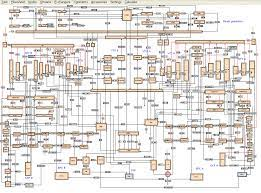
\includegraphics[width=0.75\textwidth]{figuras/RECONSET.jpg}
        \caption{Tela Principal da ferramenta RECONSET.}
        \vspace{6mm}
        \label{fig:RECONSET}
    \end{center} 
\end{figure}

O \textit{software} é orientado para PC e possui uma interface de usuário gráfica interativa, tornando-o fácil de usar. Os usuários definem problemas (ou tarefas) interativamente por meio desta interface. O RECON é capaz de equilibrar materiais e energia de componentes únicos ou múltiplos de sistemas complexos, seja em estado estacionário ou instável (dinâmico), com ou sem reações químicas (balanceamento de reatores). Além disso, ele pode realizar balanceamento de momento com base em cálculos hidráulicos de vazão em sistemas de dutos. O RECON reconcilia vazões medidas, concentrações, temperaturas e outras variáveis de processo, e calcula variáveis não medidas. Para definir um problema (ou tarefa), os usuários geralmente criam um fluxograma de processo e definem variáveis de processo, como taxas de fluxo, temperaturas, pressões, etc. O fluxograma inclui nós, fluxos de massa e energia, e trocadores de calor. Se necessário, os usuários também podem complementar (ou até mesmo substituir) o modelo de balanceamento com suas próprias equações.

\subsubsection{BILCO}

CASPEO é uma empresa francesa fundada em 2004, especializada em engenharia de processos e soluções tecnológicas. Originada do 
Departamento de Pesquisas Geológicas e Minerais da França. Ela foi criada para oferecer à indústria de mineração métodos e ferramentas computacionais resultantes de anos de pesquisa e tornou-se uma referência na indústria de processamento mineral, atendendo a vários mercados, como mineração e metalurgia, processamento de biomassa e alimentos, tratamento de resíduos sólidos e outras indústrias de processamento \cite{bilco}.

Uma das suas inovações é o \textit{software} de reconciliação de dados BILCO, projetado para derivar um balanço de material coerente e total a partir de todos os dados disponíveis (medições, análises, estimativas) para todas as correntes de processo. Ele é uma ferramenta poderosa que permite aos usuários reconciliar dados de qualquer planta de processamento, a Figura \ref{fig:BILCO}, demonstra a tela inicial do \textit{software}.

\begin{figure}[htbp!] 
    \begin{center}
        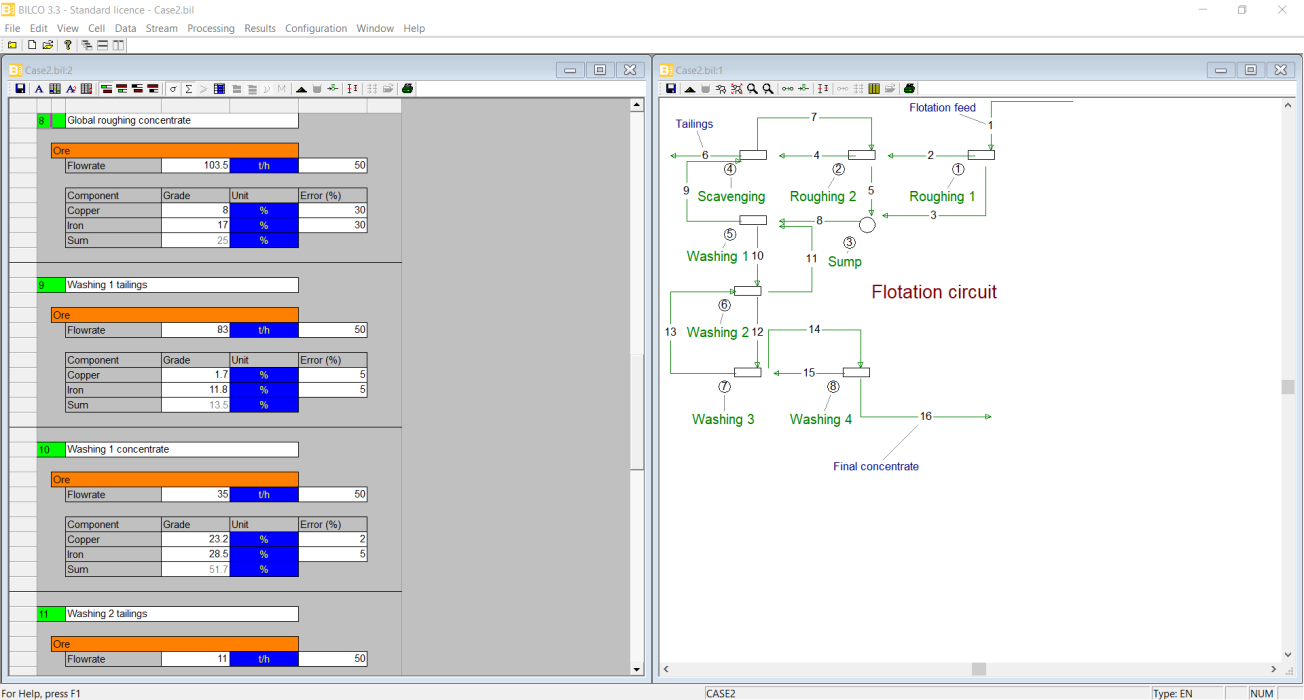
\includegraphics[width=0.75\textwidth]{figuras/BILCOCASPEOP.png}
        \caption{Tela Principal da ferramenta BILCO.}
        \vspace{6mm}
        \label{fig:BILCO}
    \end{center} 
\end{figure}

Ele tem a capacidade de se incorporar à duas outras ferramentas facilmente, no caso, à um simulador de processos, denominado USIM PAC e à um \textit{software} de contabilidade metalúrgica, INVETEO; e, dessa forma, fornece cálculos de balanço precisos e gera um conjunto de estimadores coerentes que estão em conformidades com as restrições da lei de conservação de energia, além de calcular seus erros relativos. Ele também é capaz de determinar, em quantidade e qualidade, a composição de cada corrente de processo. É um dos poucos \textit{softwares} de balanço de massa capaz de calcular toda a composição da corrente (taxas de fluxo, classes de tamanho, tipos de partículas, massa molar, etc.) em um único cálculo.

Essa solução também oferece uma única interface para gerenciar todo o processo. Consiste numa interface gráfica fácil de usar, tornando-a acessível tanto para novos usuários quanto para os mais experientes. Uma das características mais úteis do BILCO é a possibilidade de exportar os resultados para o Excel, permitindo uma análise mais profunda dos dados. Ele fornece resultados detalhados, incluindo uma planilha de comparação e uma planilha global, para uma visão completa do balanço de material.

\subsubsection{PIMSOFT}

Shorou International é uma empresa dos Emirados Árabes Unidos, que oferece soluções especializadas e serviços de engenharia com foco em automação avançada e gestão de ativos para todas as principais indústrias, com ênfase especial nos setores de petróleo, gás, utilidade e energia \cite{pimsoft}.

Uma das suas soluções é o Sistema OSIsoft PI, uma plataforma que coleta, historiza e analisa grandes quantidades de dados de séries temporais, de alta fidelidade, de várias fontes de dados e em diferentes formados. Esses dados são disponibilizados para usuários e sistemas em diversos setores de negócios. As implementações do sistema PI aproveitam o poder dos dados operacionais para gerar previsões que aumentam a consciência situacional e desencadeiam decisões bem planejadas, ajudando as empresas líderes a alcançar maiores melhorias operacionais e inovações revolucionárias em seus respectivos campos. 

E um complemento desse sistema, é o PIMSOFT SigmaFine que é um \textit{software} de verificações e balanços que utiliza princípios de conservação, estatísticas, padrões de engenharia e cálculos para monitorar e montar dados de plantas industriais. SigmaFine gera módulos coerentes, confiáveis e utilizáveis, prontos para negócios.

\subsection{Aplicação na Contabilidade}

Paralelamente à disciplina de Reconciliação de Dados na área industrial química, há uma outra área na qual investe bastante nesse campo, a de soluções contábeis. E a investigação das tendências tecnológicas emergentes é um aspecto crucial durante o processo de desenvolvimento de uma solução mais dinâmica e que consegue resolver problemas já solucionados por outras áreas da ciência.

\subsubsection{FloQast}

FloQast é uma empresa fundada em 2013, que possui uma plataforma  de contabilidade operacional baseada na nuvem, com foco em automação e gestão para uso por contadores. Uma das suas soluções é uma ferramenta de reconciliação de dados nomeada FloQast Reconciliation Management, uma solução avançada de automação de fluxo de trabalho para fornecer gerenciamento de reconciliação de contas de ponta a ponta \cite{floqast}.

Isso aumenta a velocidade e a precisão financeira do fechamento financeiro, ao mesmo tempo que gerencia o risco de declaração incorreta. Esse \textit{software} permite que controladores e suas equipes automatizem e gerenciem o processo de reconciliação de ponta a ponta, com uma solução centralizada confiável por contadores e auditores em todo o mundo.

\subsubsection{Aspen}

AspenTech, uma empresa fundada em 1981, a partir do Projeto ASPEN - uma pesquisa conjunta entre o MIT (Instituto de Tecnologia de Massachusetts) e o Departamento de Energia dos EUA na qual desenvolveu a primeira tecnologia de modelagem e simulação baseada em computador para a indústria química. Hoje, mais de 40 anos depois, com mais de 3700 funcionários e 60 localidades em todo o mundo, a empresa tem seu foco em soluções industriais, ao mesmo tempo em que enfrenta diretamente a sustentabilidade, com foco na eficiência dos recursos, transição energética, descarbonização e redução de resíduos \cite{aspen}.

Uma das suas ferramentas que utiliza soluções similares às do trabalho de conclusão de curso é a ferramenta AURA (Aspen Unified Reconciliation Accounting) uma solução que ajuda a reduzir perdas de material e aumentar margens por meio de um equilíbrio eficiente de massa e volume. Capacitando as partes interessadas a tomar melhores decisões com base em dados de produção validados e reconciliados. Sua arquitetura escalável reduz o custo total de propriedade com opções rápidas de implantação na nuvem e fácil implementação e manutenção do modelo. A precisão da reconciliação é aumentada pelo \textit{Smart Solver} proprietário que resolve automaticamente os erros de densidade medidos em laboratório. O \textit{software} também ajuda a atingir metas de redução de emissões ao automatizar o rastreamento, monitoramento e relatórios de emissões de gases de efeito estufa e intensidade de carbono do produto. Além disso, permite fechar o balanço mais rapidamente com fluxos de trabalho intuitivos, interpretação fácil dos resultados com visualização avançada e relatórios dinâmicos poderosos.


% ---

\subsection{Pesquisas Sendo Desenvolvidas}

O objetivo do RADARE é incorporar avanços tecnológicos de diversas áreas, com foco não apenas nas técnicas aplicadas diretamente à reconciliação de dados, mas também em áreas adjacentes que possam contribuir para o aprimoramento da ferramenta. Dessa forma, é fundamental estar alinhado com as pesquisas mais recentes em reconciliação de dados computacional, bem como explorar como elas podem ser aplicadas no contexto industrial brasileiro.

Pesquisas em outras áreas de aplicação, como o processamento mineral e a distribuição de gás, também oferecem contribuições valiosas para o desenvolvimento do RADARE, especialmente na aplicação de técnicas de reconciliação de dados em diferentes cenários industriais.

\subsubsection{Controle e Supervisão de Processamento Mineral}

A pesquisa apresentada por Daniel Hoduin \cite{danielhoduin} foca nas restrições de conservação de massa e energia, que servem como base para o desenvolvimento de estratégias de medição, atualização do valor medido por meio de técnicas de filtragem de erros de medição e estimativa de variáveis de processo não medidas. Nas unidades de processamento mineral, as principais variáveis são geralmente as vazões e concentrações, e a reconciliação desses dados com as leis de conservação de massa é essencial para manter a precisão dos processos.

Os métodos de reconciliação propostos utilizam técnicas clássicas, como os mínimos quadrados usuais, que minimizam os erros entre os valores observados e os valores estimados. Além disso, a filtragem de Kalman, um algoritmo de estimação recursiva, é empregada para estimar variáveis de estado de processos dinâmicos e com ruído. São sugeridas ferramentas para três tipos de regimes operacionais: regime estacionário, quase-estacionário e dinâmico.

As ferramentas propostas para diferentes regimes operacionais de processamento mineral podem ser adaptadas para o RADARE, permitindo que ele lide com cenários variáveis de fluxo de dados e oferecendo maior flexibilidade no tratamento de dados de processos industriais com características dinâmicas.

\subsubsection{Balanços de Materiais em Rede de Distribuição de Gás}

O desenvolvimento realizado por Jesús David Badillo Herrera, Arlex Chaves e José Augusto Fuentes Osorio \cite{balancecontrol}, foca em uma solução prática para enfrentar os desafios apresentados por erros em sistemas de distribuição de gás natural. A ferramenta combina técnicas numéricas e estatísticas, como a Reconciliação de Dados (DR) e a Detecção de Erros Brutos (GED), para melhorar a precisão das medições e garantir a conformidade com as leis de conservação de massa.

Essa abordagem não apenas aprimora a acurácia das medições, mas também identifica e corrige erros grosseiros, proporcionando maior confiabilidade nos dados. A validação da ferramenta com problemas da literatura e sua aplicação em uma rede de distribuição real demonstram sua eficácia em fornecer resultados reconciliados com alta precisão.

A abordagem combinada de Reconciliação de Dados (DR) e Detecção de Erros Brutos (GED), utilizada na distribuição de gás natural, foi ser integrada ao RADARE para garantir maior precisão nas medições e identificar rapidamente inconsistências ou erros em sistemas industriais.

% ---

\section{Justificativa}

O setor industrial brasileiro, responsável por uma parcela significativa da economia nacional, enfrenta desafios críticos relacionados à qualidade e confiabilidade dos dados gerados em processos produtivos. A falta de precisão nas medições e a ausência de ferramentas eficazes para a reconciliação de dados comprometem a eficiência operacional e a competitividade das indústrias. Dessa forma, torna-se urgente o desenvolvimento de soluções tecnológicas que possam superar essas limitações, sendo o \textit{software} RADARE uma proposta que visa preencher essa lacuna com inovação e eficácia.

A escolha por desenvolver o RADARE como uma aplicação \textit{web} é estratégica, pois o ambiente web oferece diversas vantagens essenciais para o setor industrial. Entre elas, a interoperabilidade eficiente entre sistemas permite integrar o \textit{software} com outras ferramentas já utilizadas nas plantas industriais. O acesso remoto possibilita que engenheiros e operadores possam monitorar e controlar os processos de qualquer localidade, reduzindo tempos de inatividade e melhorando a resposta a problemas. Além disso, a facilidade de uso da plataforma, associada à alta acessibilidade para indivíduos com necessidades especiais, amplia o alcance da solução, garantindo que o sistema possa ser adotado por uma gama diversa de usuários.

O projeto RADARE visa atender a uma demanda crescente por soluções no setor industrial brasileiro, onde a competitividade global exige maior eficiência e qualidade nas operações. O contexto brasileiro apresenta desafios específicos, como a falta de ferramentas acessíveis e adaptadas à realidade das indústrias locais. O RADARE se diferencia por ser uma solução criada para o contexto nacional, ao mesmo tempo em que incorpora tecnologias de ponta e metodologias comprovadas internacionalmente, como o método dos multiplicadores de Lagrange, aplicado de forma inovadora em uma plataforma web de fácil acesso e integração.

O RADARE representa uma inovação ao unir teorias avançadas de reconciliação de dados com tecnologias modernas de desenvolvimento \textit{web}. Ao criar uma solução que é tanto acessível quanto adaptável às necessidades do setor industrial, o RADARE tem o potencial de impactar diretamente a eficiência das operações industriais no Brasil, promovendo o desenvolvimento tecnológico e aumentando a competitividade das empresas brasileiras no cenário global.

Este trabalho está estruturado da seguinte forma: no Capítulo 1, apresenta-se a introdução, contextualizando o problema e destacando os objetivos principais e secundários da pesquisa. O Capítulo 2 oferece o referencial teórico, com definições e descrições das principais teorias que embasam a solução proposta. No Capítulo 3, descrevem-se os métodos e técnicas utilizados para o desenvolvimento do sistema, assim como o cronograma de atividades apresentado por meio do diagrama de Gantt. Por fim, no Capítulo 4, são feitas as considerações finais sobre o aprendizado adquirido, as reflexões sobre os resultados esperados no desenvolvimento futuro do projeto e as contribuições gerais da pesquisa.

% ------------------------- REVISADO - GRAMATICA - CITAÇÃO
\mychapter{Referencial teórico}
\label{Cap:ReferencialTeorico}

Este capítulo explora a prática da reconciliação de dados, a sua aplicação no âmbito industrial e a utilização da técnica de minimização de multivariáveis pelo método de multiplicadores de Lagrange, que servem como base para o desenvolvimento do \textit{software} apresentado. Além disso, discute-se o desenvolvimento de uma plataforma \textit{web} que proporciona acessibilidade e praticidade para o monitoramento e a manipulação de dados em tempo real. O capítulo contextualiza ainda a sinergia entre a indústria e a internet, destacando o papel essencial que a plataforma \textit{web} desempenha no cenário atual ao integrar técnicas de reconciliação com uma interface intuitiva e acessível.

% ------------------------- REVISADO - GRAMATICA - CITAÇÃO
\section{Reconciliação de dados e método de Lagrange}

% ------------------------- REVISADO - GRAMATICA - CITAÇÃO
\subsection{Definição de reconciliação de dados}

A reconciliação de dados é uma prática utilizada em diversas áreas da ciência e engenharia para assegurar a consistência e precisão dos dados provenientes de diferentes fontes \cite{datarecshakar}. Em contextos como sistemas industriais, processos químicos e redes de sensores, essa técnica é essencial para garantir que os dados coletados estejam alinhados e coerentes. Basicamente, a reconciliação de dados envolve comparar e corrigir discrepâncias entre os valores observados e os valores esperados, com base em modelos e relações matemáticas predefinidas \cite{datarecragnoli}.

Com a evolução dos sistemas automatizados de coleta de dados, como PLCs, sistemas supervisórios e PIMS \cite{plcsupervisory2021}, a captura e o encaminhamento de dados tornaram-se processos eficientes. No entanto, muitos desses dados não satisfazem as equações de balanço, fundamentais em contextos industriais \cite{balance2020}. De acordo com essas equações, em um contorno fechado, a soma das saídas deve ser igual à soma das entradas, subtraindo-se o valor acumulado:

\begin{equation}
	\sum (\text{saídas}) = \sum (\text{entradas}) - \text{armazenado}
\end{equation}

Essa inconsistência geralmente decorre de fatores como erros de medição aleatórios, instrumentos descalibrados, modelagem inadequada e frequências incorretas de amostragem \cite{measurementerror2020}. Outros fatores, como a variação de densidade devido à temperatura e leituras fora da faixa de operação dos instrumentos, também contribuem para esses desvios \cite{temperaturedensity2022}.

Tradicionalmente, os ajustes nos dados baseiam-se em níveis de confiança atribuídos empiricamente a determinadas medições, o que envolve ajustes manuais e subjetivos \cite{empiricaladjustment2023}. No entanto, o presente trabalho busca introduzir uma abordagem matemática para recalcular os valores mais prováveis, eliminando a dependência de ajustes empíricos e subjetivos e promovendo uma análise mais objetiva e fundamentada dos dados industriais \cite{mathematicalapproach2024}.

% ------------------------- REVISADO - GRAMATICA - CITAÇÃO
\subsection{Reconciliação de dados no âmbito industrial}

No começo da década de 1960 se entendeu a importância do controle de processos químicos industriais por computadores que aplicavam técnicas matemáticas \cite{computecontrol}, dessa forma surge a área da computação voltada à reconciliação de dados, na qual há a comparação, validação e correção de informações coletadas em diferentes pontos do processo, a fim de determinar a consistência dos dados, a qualidade dos mesmos ou até otimizar os processos \cite{datarecshakar}.

Ao longo das últimas décadas, os métodos de reconciliação de dados evoluíram significativamente, acompanhando os avanços tecnológicos e as demandas crescentes da indústria \cite{datarecsurvey}. Com o advento de sistemas de automação mais avançados, sensores inteligentes e a proliferação de dispositivos conectados, a quantidade de dados gerados nas operações industriais aumentou drasticamente \cite{datarecsurvey}. Nesse contexto, a reconciliação, análise e gestão de dados tornaram-se ferramentas indispensáveis para garantir a integridade e a confiabilidade das informações coletadas em tempo real \cite{aularecon}.

Na era contemporânea, a reconciliação de dados desempenha um papel crucial na otimização dos processos industriais, contribuindo para a eficiência operacional e a redução de custos. Sistemas avançados de reconciliação não apenas comparam e validam dados, mas também utilizam algoritmos sofisticados para identificar padrões, tendências e anomalias \cite{datarecragnoli}. Essa capacidade analítica permite que as indústrias ajam proativamente, antecipando-se a problemas potenciais, otimizando a produção e melhorando a qualidade dos produtos finais \cite{datarecshakar}.

% ------------------------- REVISADO - GRAMATICA - CITAÇÃO
\subsection{Minimização de Multivariáveis por Multiplicadores de Lagrange}

A técnica de minimização por multiplicadores de Lagrange foi introduzida por Joseph-Louis Lagrange, um matemático e físico francês nascido em 25 de janeiro de 1736, em Turim, Itália, que mais tarde se estabeleceu na França. Lagrange é conhecido por suas contribuições fundamentais em mecânica analítica, cálculo e teoria dos números, além de desenvolver o método dos multiplicadores de Lagrange no século XVIII, fornecendo uma maneira eficaz de resolver problemas de otimização condicionada \cite{lagrange}.

% ------------------------- REVISADO - GRAMATICA - CITAÇÃO
\subsubsection{O método dos multiplicadores de Lagrange}

O método dos multiplicadores de Lagrange é uma técnica utilizada para encontrar máximos e mínimos de uma função sujeita a uma ou mais restrições. Considera-se o problema de minimizar uma função $f(x, y, z, \dots)$ sujeita a uma restrição $g(x, y, z, \dots) = 0$. Para transformar esse problema com restrições em um problema sem restrições, introduz-se uma variável adicional, o multiplicador de Lagrange, que representa o impacto da restrição sobre a função objetivo. Em um problema de minimização com uma única restrição, a função de Lagrange $\mathcal{L}$ é definida como mostrado na Equação \ref{eq
}:

\begin{equation} \mathcal{L}(x, y, z, \dots, \lambda) = f(x, y, z, \dots) + \lambda \cdot g(x, y, z, \dots) \label{eq
} \end{equation}

onde $\lambda$ é o multiplicador de Lagrange.

A solução do problema ocorre ao determinar os pontos críticos de $\mathcal{L}$, isto é, os pontos onde as derivadas parciais de $\mathcal{L}$ em relação a todas as variáveis (incluindo $\lambda$) são iguais a zero. Portanto, é necessário resolver o sistema de equações conforme apresentado na Equação \ref{eq:lambdaa}:

\begin{equation} \frac{\partial \mathcal{L}}{\partial x} = 0, \quad \frac{\partial \mathcal{L}}{\partial y} = 0, \quad \frac{\partial \mathcal{L}}{\partial z} = 0, \quad \dots, \quad \frac{\partial \mathcal{L}}{\partial \lambda} = 0 \label{eq:lambdaa} \end{equation}

% ------------------------- REVISADO - GRAMATICA - CITAÇÃO
\subsubsection{Exemplo com duas variáveis}

Considera-se o caso de uma função de duas variáveis, $f(x, y)$, que necessita ser minimizada sujeita a uma restrição $g(x, y) = 0$. A função de Lagrange é dada por:

\begin{equation}
	\mathcal{L}(x, y, \lambda) = f(x, y) + \lambda \cdot g(x, y)
	\label{eq:lagrange_two_variable}
\end{equation}

Para encontrar os valores de $x$, $y$ e $\lambda$ que minimizam $f(x, y)$, resolve-se o sistema de equações apresentado nas Equações \ref{eq:partial_x}, \ref{eq:partial_y} e \ref{eq:partial_lambda}, conforme mostrado a seguir:

\begin{equation}
	\frac{\partial \mathcal{L}}{\partial x} = \frac{\partial f}{\partial x} + \lambda \frac{\partial g}{\partial x} = 0
	\label{eq:partial_x}
\end{equation}
\begin{equation}
	\frac{\partial \mathcal{L}}{\partial y} = \frac{\partial f}{\partial y} + \lambda \frac{\partial g}{\partial y} = 0
	\label{eq:partial_y}
\end{equation}
\begin{equation}
	\frac{\partial \mathcal{L}}{\partial \lambda} = g(x, y) = 0
	\label{eq:partial_lambda}
\end{equation}

A resolução desse sistema fornece os valores de $x$, $y$ e $\lambda$ que minimizam $f(x, y)$ enquanto satisfazem a restrição $g(x, y) = 0$.

O método dos multiplicadores de Lagrange é amplamente utilizado em diversas áreas, incluindo otimização de processos industriais, economia e física, onde os problemas frequentemente envolvem restrições complexas. A abordagem permite uma solução sistemática e rigorosa para problemas de otimização condicionada, assegurando que as soluções encontradas respeitem as restrições impostas \cite{lagrangeoptbook}.

% ------------------------- REVISADO - GRAMATICA - CITAÇÃO
\subsection{Aplicação do método dos multiplicadores de Lagrange à necessidade de reconciliação de dados}

Para resolver o problema de balanço de massas, o método dos multiplicadores de Lagrange é aplicado adotando o critério dos mínimos quadrados. Define-se uma função objetivo a ser minimizada, que corresponde à soma ponderada dos quadrados dos erros nas medições.

Seja $M_i$ o valor medido de um fluxo e $\hat{M}_i$ o valor corrigido para o mesmo fluxo. O erro $E_i$ é então definido como a diferença entre esses valores, conforme a Equação (5.7):
\begin{equation}
	E_i = M_i - \hat{M}_i
\end{equation}

O erro quadrático correspondente é dado pela Equação (5.8):
\begin{equation}
	E_i^2 = (M_i - \hat{M}_i)^2
\end{equation}

Para ponderar cada erro, utiliza-se o inverso do desvio padrão associado à medida. A função objetivo, portanto, é formulada da seguinte maneira, como demonstrado na Equação (5.9):
\begin{equation}
	F(\hat{M}_1, \hat{M}_2, \dots, \hat{M}_n) = \sum_{i=1}^n \frac{(M_i - \hat{M}_i)^2}{\sigma_i^2}
\end{equation}

As restrições para o problema são expressas pela Equação (5.10):
\begin{equation}
	\phi_j(\hat{M}_1, \hat{M}_2, \dots, \hat{M}_n) = 0, \quad j = 1, 2, \dots, m
\end{equation}
onde cada $\phi_j$ representa uma equação de balanço de massa para um nodo do circuito, totalizando $m$ equações de restrição.

A função de Lagrange, que incorpora essas restrições, é então definida pela Equação (5.11):
\begin{equation}
	\Phi = \sum_{i=1}^n \frac{(M_i - \hat{M}_i)^2}{\sigma_i^2} + \sum_{j=1}^m \lambda_j \phi_j(\hat{M}_1, \hat{M}_2, \dots, \hat{M}_n)
\end{equation}

Calculando as derivadas parciais de $\Phi$ em relação a cada variável corrigida $\hat{M}_i$ e igualando a zero, obtem-se um conjunto de $n$ equações para cada medida, como mostrado na Equação (5.12):
\begin{equation}
	\frac{\partial \Phi}{\partial \hat{M}_1} = 0, \quad \frac{\partial \Phi}{\partial \hat{M}_2} = 0, \quad \dots, \quad \frac{\partial \Phi}{\partial \hat{M}_n} = 0
\end{equation}

Juntas com as $m$ equações de restrição $\phi_j = 0$, essas expressões formam um sistema de $n + m$ equações para $n + m$ incógnitas, permitindo a resolução para determinar os valores reconciliados das variáveis.

% ------------------------- REVISADO - GRAMATICA - CITAÇÃO
\subsubsection{Exemplo com um problema de balanço de sistema}
Para ilustrar a aplicação do método dos multiplicadores de Lagrange na reconciliação de dados, considera-se um problema de balanço de um sistema com o número de medições \(N = 3\) e o número de nodos \(H = 1\), descrito na Figura \ref{Fig:ExemploImage}.

\begin{figure}[htbp]
    \centering
    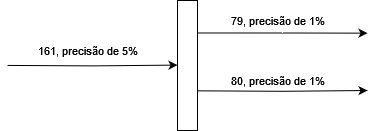
\includegraphics[width=0.6\textwidth]{figuras/exemplo-problema.png}
    \caption{Um exemplo com medidas (Fonte: próprio autor, 2024).}
    \label{Fig:ExemploImage}
\end{figure}

O vetor de medições \(m\) é dado pela Equação \eqref{eq:medidas}:
\begin{equation}
    m = [M_1 \quad M_2 \quad M_3] = [161 \quad 79 \quad 80]
    \label{eq:medidas}
\end{equation}

O vetor de desvios percentuais \(p\) é expresso na Equação \eqref{eq:desvios_percentuais}:
\begin{equation}
    p = [\sigma_1 \quad \sigma_2 \quad \sigma_3] = [0.05 \quad 0.01 \quad 0.01]
    \label{eq:desvios_percentuais}
\end{equation}

Para calcular o vetor de desvios absolutos \(a\), utiliza-se a notação do Matlab, realizando a operação elemento a elemento entre o vetor de medições e o vetor de desvios percentuais, conforme demonstrado na Equação \eqref{eq:desvios_absolutos}:
\begin{equation}
    a = m .* p = [8.05 \quad 0.79 \quad 0.80]
    \label{eq:desvios_absolutos}
\end{equation}

Para facilitar a implementação do cálculo de reconciliação, o sistema é formulado em notação matricial. A Equação \eqref{eq:sistema_matricial} representa o sistema de equações utilizado:

\begin{equation}
\begin{bmatrix}
    \frac{2}{a_1^2} & 0 & 0 & 1 \\
    0 & \frac{2}{a_2^2} & 0 & -1 \\
    0 & 0 & \frac{2}{a_3^2} & 1 \\
    1 & -1 & -1 & 0 \\
\end{bmatrix}
\begin{bmatrix}
    \hat{M}_1 \\
    \hat{M}_2 \\
    \hat{M}_3 \\
    \lambda_1 \\
\end{bmatrix}
=
\begin{bmatrix}
    \frac{2 M_1}{a_1^2} \\
    \frac{2 M_2}{a_2^2} \\
    \frac{2 M_3}{a_3^2} \\
    0 \\
\end{bmatrix}
\label{eq:sistema_matricial}
\end{equation}

A resolução do sistema, conforme mostrado na Equação \eqref{eq:sistema_resolvido}, é realizada invertendo a matriz e multiplicando-a pelo vetor dos termos independentes:

\begin{equation}
\begin{bmatrix}
    \hat{M}_1 \\
    \hat{M}_2 \\
    \hat{M}_3 \\
    \lambda_1 \\
\end{bmatrix}
=
\begin{bmatrix}
    \frac{2}{a_1^2} & 0 & 0 & 1 \\
    0 & \frac{2}{a_2^2} & 0 & -1 \\
    0 & 0 & \frac{2}{a_3^2} & 1 \\
    1 & -1 & -1 & 0 \\
\end{bmatrix}^{-1}
\begin{bmatrix}
    \frac{2 M_1}{a_1^2} \\
    \frac{2 M_2}{a_2^2} \\
    \frac{2 M_3}{a_3^2} \\
    0 \\
\end{bmatrix}
\label{eq:sistema_resolvido}
\end{equation}

O vetor de correções, que representa as diferenças entre as medições originais e os valores reconciliados, é definido pela Equação \eqref{eq:vetor_correcoes}:

\begin{equation}
\begin{bmatrix}
    E_1 \\
    E_2 \\
    E_3 \\
\end{bmatrix}
=
\begin{bmatrix}
    M_1 \\
    M_2 \\
    M_3 \\
\end{bmatrix}
-
\begin{bmatrix}
    \hat{M}_1 \\
    \hat{M}_2 \\
    \hat{M}_3 \\
\end{bmatrix}
\label{eq:vetor_correcoes}
\end{equation}

O resultado final das medidas reconciliadas é apresentado na Equação \eqref{eq:medidas_reconciliadas}:

\begin{equation}
    Rec = [159.0383 \quad 79.0189 \quad 80.0194]
    \label{eq:medidas_reconciliadas}
\end{equation}

A correção dos valores, ou seja, a variação entre o valor medido e o valor reconciliado, é descrita na Equação \eqref{eq:correcao_valores}:

\begin{equation}
    E = [1.9617 \quad -0.0189 \quad -0.0194 ]
    \label{eq:correcao_valores}
\end{equation}



% ------------------------- REVISADO - GRAMATICA - CITAÇÃO
\section{Desenvolvimento de um \textit{software online}}

O desenvolvimento de \textit{softwares} online modernos requer uma abordagem estruturada que combina diferentes áreas de conhecimento, como \textit{front-end}, \textit{back-end} e gerenciamento de banco de dados. Esses componentes trabalham em conjunto para criar sistemas robustos, escaláveis e acessíveis, fundamentais para atender às demandas de aplicações na \textit{web}.

% ------------------------- REVISADO - GRAMATICA - CITAÇÃO
\subsection{Desenvolvimento \textit{Front-End}}

O \textit{front-end} é a camada de uma aplicação com a qual os usuários interagem diretamente. Ele compreende os elementos visíveis e interativos da interface, como botões, menus, e formulários, e é fundamental para proporcionar uma experiência de uso intuitiva e eficiente \cite{frontendrole}. O desenvolvimento de um \textit{front-end} eficaz exige atenção tanto à organização visual quanto à responsividade, garantindo que a aplicação funcione bem em diferentes dispositivos e tamanhos de tela.

Para o desenvolvimento \textit{front-end}, existem diversas linguagens e \textit{frameworks} amplamente utilizados. HTML, CSS e JavaScript são as linguagens fundamentais para a construção de interfaces web. Entre os \textit{frameworks} e bibliotecas mais populares estão \textit{React}, \textit{Vue.js} e \textit{Angular}, que oferecem ferramentas avançadas para criar interfaces de usuário dinâmicas e reativas \cite{reactbook}. Além disso, \textit{frameworks} de estilo como \textit{Bootstrap} e \textit{Tailwind CSS} auxiliam no \textit{design} responsivo e na organização visual das páginas \cite{bootstrapdoc}.

No desenvolvimento do RADARE, a construção da interface foi realizada utilizando \textit{TypeScript} em conjunto com HTML e SCSS, proporcionando uma base sólida para a criação de interfaces organizadas e responsivas \cite{typescriptbook}. O HTML foi utilizado para estruturar os elementos visuais da interface, enquanto o SCSS garantiu um controle avançado sobre o \textit{design} e o estilo, permitindo uma customização precisa de cada componente \cite{htmlcssbook}. A escolha do \textit{TypeScript} trouxe benefícios como tipagem estática e maior segurança no desenvolvimento, facilitando a criação de uma interface robusta e escalável \cite{typescriptsecurity}. Diferente do uso de \textit{frameworks} de \textit{front-end}, que adicionam camadas adicionais de abstração, a combinação direta dessas tecnologias possibilitou um controle detalhado sobre a interface e a experiência do usuário \cite{frontendwithoutframework}.

% ------------------------- REVISADO - GRAMATICA - CITAÇÃO
\subsection{Desenvolvimento \textit{Back-End}}

O \textit{back-end} de uma aplicação é a parte que opera "por trás dos panos", onde toda a lógica de negócios, manipulação de dados e comunicação com o banco de dados ocorre. Essa camada é fundamental para o funcionamento adequado do sistema, pois realiza operações como autenticação, processamento de dados e execução de cálculos específicos, garantindo que as informações exibidas no \textit{front-end} estejam sempre atualizadas e em conformidade com as regras de negócio definidas \cite{backendroles}.

Entre as linguagens mais utilizadas para o desenvolvimento de \textit{back-end} estão \textit{Python}, \textit{Java}, \textit{Ruby}, \textit{PHP}, e \textit{Node.js}. Cada uma delas possui características específicas que se adequam a diferentes tipos de aplicações e requisitos de desempenho, escalabilidade e manutenção \cite{backendlanguages}. Por exemplo, a linguagem \textit{Python} é amplamente apreciada por sua sintaxe clara e suporte a bibliotecas de manipulação de dados, enquanto \textit{Java} é conhecida por sua robustez e escalabilidade em grandes sistemas empresariais \cite{javabackend}.

No desenvolvimento do RADARE, o \textit{back-end} foi inteiramente construído utilizando a linguagem \textit{Python}, que permite a implementação de uma estrutura eficiente para manipulação de dados e integração com o \textit{front-end} \cite{pythonweb}. Com a \textit{Python}, é possível desenvolver APIs que facilitam a comunicação entre a interface de usuário e o sistema de armazenamento de dados, garantindo uma troca eficiente de informações e a consistência dos dados processados \cite{pythonapi}. A linguagem também forneceu um ambiente propício para lidar com a lógica de reconciliação de dados, pois realiza operações necessárias de forma otimizada e segura \cite{pythondata}.

Por meio dessa abordagem, o \textit{back-end} do RADARE é capaz de processar dados de entrada, realizar cálculos de reconciliação e enviar os resultados para o \textit{front-end} de maneira integrada \cite{backendworkflow}. Esse uso exclusivo de \textit{Python} como linguagem \textit{back-end} trouxe simplicidade e consistência ao sistema, atendendo aos requisitos do projeto com robustez e flexibilidade.

% ------------------------- REVISADO - GRAMATICA - CITAÇÃO
\subsection{Desenvolvimento do banco de dados}

Um banco de dados é uma coleção organizada de informações estruturadas, geralmente armazenadas e acessadas eletronicamente a partir de um sistema de computador. Em sistemas modernos, os bancos de dados são essenciais para armazenar, recuperar e gerenciar grandes volumes de dados de maneira rápida e eficiente. Eles desempenham um papel central em aplicações \textit{online}, onde a integridade, consistência e segurança dos dados são fundamentais.

Existem diferentes tipos de bancos de dados, cada um projetado para atender a requisitos específicos de armazenamento e acesso. Entre os modelos mais comuns estão dois:

\begin{itemize}
	\item \textbf{Bancos de dados relacionais (SQL)}: Organizam os dados em tabelas com linhas e colunas, permitindo consultas complexas através da linguagem SQL. Exemplos incluem \textit{PostgreSQL}, \textit{MySQL} e \textit{Oracle Database} \cite{relationaldatabases}.

	\item \textbf{Bancos de dados não relacionais(NoSQL)}: Projetados para armazenamento flexível de dados não estruturados ou semi-estruturados, esses bancos de dados não utilizam a estrutura tradicional de tabelas. São divididos em subcategorias como \textit{document stores} (ex.: \textit{MongoDB}), \textit{key-value stores} (ex.: \textit{Redis}), \textit{column stores} (ex.: \textit{Cassandra}) e \textit{graph databases} (ex.: \textit{Neo4j}) \cite{nosqldatabases}.
\end{itemize}

No desenvolvimento do RADARE, o banco de dados foi implementado utilizando exclusivamente o \textit{PostgreSQL}, um sistema de gerenciamento de banco de dados relacional robusto e altamente confiável \cite{postgresql2024}. O \textit{PostgreSQL} foi escolhido por sua capacidade de gerenciar grandes volumes de dados e por oferecer suporte a transações complexas, garantindo a integridade e consistência das informações armazenadas \cite{acidtransactions}.

O \textit{PostgreSQL} organiza os dados em tabelas relacionais, onde cada linha e coluna representam uma entidade específica e suas respectivas propriedades, facilitando a execução de consultas e manipulações complexas \cite{relationaldatabases}. Além disso, o sistema fornece mecanismos de integridade referencial, que ajudam a manter a consistência dos dados por meio de relações entre tabelas \cite{databaseintegrity}. Essa estrutura é essencial para a reconciliação de dados, uma vez que permite organizar e recuperar informações de forma rápida e precisa.

% ------------------------- REVISADO - GRAMATICA - CITAÇÃO
\subsection{Metodologias de desenvolvimento de \textit{software}}

O desenvolvimento de \textit{software} moderno conta com metodologias específicas que auxiliam na organização, planejamento e execução dos projetos, permitindo maior controle sobre prazos, custos e qualidade do produto final. Entre as metodologias mais utilizadas estão as abordagens ágeis, que buscam otimizar a comunicação entre as equipes e permitir a adaptação contínua aos requisitos do cliente ao longo do ciclo de desenvolvimento.

\begin{itemize} \item \textbf{Agile}: Agile é uma abordagem de desenvolvimento de \textit{software} que se concentra na flexibilidade e na capacidade de adaptação rápida a mudanças nos requisitos \cite{agilemanif}. A metodologia foi formalizada pelo Manifesto Agile em 2001, propondo valores como colaboração com o cliente, resposta a mudanças e entrega contínua de \textit{software} funcional. Em vez de desenvolver o produto como um todo, as equipes Agile dividem o projeto em pequenos incrementos, denominados \textit{sprints}, para gerar valor continuamente ao cliente \cite{agilepractices}.

    \item \textbf{Scrum}: Scrum é uma estrutura dentro da metodologia Agile que organiza o desenvolvimento em \textit{sprints} de curta duração, geralmente de duas a quatro semanas \cite{scrumguide}. Durante cada \textit{sprint}, a equipe trabalha em um conjunto específico de tarefas, definido em uma reunião de planejamento. Ao final de cada ciclo, ocorre uma reunião de revisão onde o progresso é avaliado e ajustes são feitos para o próximo \textit{sprint}. O Scrum enfatiza papéis específicos, como o \textit{Scrum Master} e o \textit{Product Owner}, para manter a equipe focada e produtiva \cite{scrumroles}.

	\item \textbf{Kanban}: Kanban é uma metodologia visual que utiliza um quadro dividido em colunas para representar o fluxo de trabalho, permitindo a gestão e otimização das tarefas \cite{kanbanmethod}. Com foco na melhoria contínua e na redução de desperdícios, o Kanban permite que a equipe ajuste a quantidade de trabalho em progresso para evitar sobrecarga. Essa metodologia é particularmente útil em ambientes onde as tarefas variam constantemente e é necessária uma alta adaptabilidade \cite{kanbanflow}.

	\item \textbf{Extreme Programming (XP)}: O XP é uma metodologia que enfatiza a excelência técnica e práticas rigorosas de desenvolvimento, como programação em par, desenvolvimento orientado a testes (TDD) e integração contínua \cite{extremeprogramming}. O XP visa melhorar a qualidade do \textit{software} e a capacidade de resposta a mudanças, focando na colaboração constante com o cliente e em entregas frequentes de pequenas funcionalidades \cite{tddxp}.

\end{itemize}

Essas metodologias oferecem ferramentas e práticas que ajudam as equipes de desenvolvimento a gerenciar e controlar o progresso dos projetos de \textit{software}, permitindo entregas consistentes e satisfatórias para os clientes. A escolha de uma metodologia específica depende dos requisitos do projeto, da estrutura da equipe e da cultura organizacional, sendo fundamental para o sucesso e a qualidade do produto final.

% ------------------------- REVISADO
\section{A sinergia entre a indústria e a internet}

O panorama atual de avanço da internet e a convergência entre a internet e o setor industrial representam um marco significativo na era da Engenharia de Computação \cite{industry4status}. Este fenômeno transformador tem sido impulsionado pela fusão das tecnologias da informação com os processos industriais, dando origem a conceitos como Indústria 4.0.

No âmbito desta ferramenta, é aplicada a intersecção dessas duas esferas, onde os conceitos de práticas industriais, reconciliação, análise e qualidade de dados se integram à internet, na qual é extraído deles o seu maior forte, como uma maior integralidade com outros sistemas por meio de APIs (interfaces de programação de aplicativos), melhor interatividade entre os elementos do sistema, promovendo uma comunicação mais dinâmica e eficaz, aumento da eficiência operacional e facilidade na gestão de processos \cite{industry4}. Essa sinergia possibilita a criação de ecossistemas industriais mais conectados nos quais os dados relevantes podem ser tratados de forma segura e eficiente. \cite{industrybuild}.

O horizonte atual, delineado pelos recentes avanços tecnológicos e inovações sustenta a perspectiva otimista que as indústrias estão destinadas a experimentar um crescimento substancial no país \cite{industrychina}. A convergência entre a internet e o setor industrial representa um catalisador significativo para a modernização e eficiência operacional. A integração de práticas avançadas de desenvolvimento de soluções voltadas à usabilidade e ao ambiente de desenvolvimento com controle computacional, como a reconciliação de dados e análise preditiva, impulsiona a qualidade e consistência dos processos produtivos \cite{industrydigital}.

Além disso, a aplicação da internet nas práticas industriais não só fortalece a competitividade das empresas, mas também desempenha um papel crucial na expansão econômica do país \cite{industryiot}. A capacidade de adotar tecnologias inovadoras como a automação avançada, coloca as indústrias em uma posição estratégica para atender às crescentes demandas do mercado e elevar a produtividade \cite{industryinternet}. Nesse sentido é plausível afirmar que, diante do atual cenário tecnológico e das tendências emergentes, a ferramenta desenvolvida nesse trabalho tem um grande potencial para aplicação industrial e que pode ajudar a solucionar um problema existente.
TODO
- Adicionar pesquisa sobre paleta de cores e resultados

\mychapter{Metodologia}
\label{Cap:Metodologia}

Este capítulo aborda a metodologia aplicada no desenvolvimento do \textit{software}, quais métodos de engenharia de \textit{software} foram aplicados durante o processo, desde a concepção, até a prototipação

\section{Metodologia de Desenvolvimento do RADARE}

O desenvolvimento do \textit{software} RADARE adotou o método ágil Scrum como estrutura principal para orientar o processo de criação e entrega do produto \cite{softwareengreq}. Ele sendo uma metodologia ágil amplamente reconhecida, escolhido devido à sua capacidade de promover uma abordagem iterativa e flexível, especialmente adequada para uma equipe com um único desenvolvedor, como é o caso do desenvolvimento do RADARE \cite{scrum}.

\subsection{Descrição do método Scrum}

Scrum é uma metodologia ágil de desenvolvimento de \textit{software} que enfatiza a entrega iterativa e incremental de funcionalidades. Apesar de ter sido projetado para equipes multidisciplinares, pode ser adaptado para uma equipe de um só desenvolvedor devido aos seus princípios flexíveis e foco na entrega contínua de valor \cite{scrumlove}.
        
No Scrum, o trabalho é dividido em ciclos de desenvolvimento chamados de \textit{sprints}, geralmente com duração de duas a quatro semanas. Cada \textit{sprints} começa com uma reunião de planejamento, onde o desenvolvedor define as metas e prioridades do \textit{sprints} com base nas necessidades do projeto \cite{scrummic}. Durante o \textit{sprint}, o desenvolvedor trabalha na implementação das funcionalidades definidas no planejamento. O progresso é monitorado diariamente em reuniões curtas chamadas de \textit{daily scrums}, onde o desenvolvedor atualiza a equipe sobre o seu progresso, identifica quaisquer impedimentos e ajusta o plano conforme necessário. Ao final de cada \textit{sprint}, o desenvolvedor realiza uma revisão do \textit{sprint}, demonstrando as funcionalidades concluídas à equipe ou ao cliente, e uma retrospectiva do \textit{sprint}, identificando o que funcionou bem e o que pode ser melhorado no próximo \textit{sprint} \cite{scrumproj}.
        
Esse método de desenvolvimento de \textit{software} é funcional mesmo para equipes de um só desenvolvedor, promovendo uma abordagem colaborativa, adaptativa e transparente, permitindo que o desenvolvedor mantenha um alto nível de visibilidade e controle sobre o progresso do projeto. A abordagem iterativa e incremental do Scrum também facilita a adaptação a mudanças nos requisitos do projeto e permite que o desenvolvedor entregue continuamente valor de forma mais rápida e frequente ao cliente, ou orientador, no caso do RADARE \cite{scrum}.
        
\subsubsection{Aplicação do método Scrum no Desenvolvimento do \textit{Software} RADARE}

Ao utilizar o Scrum, o desenvolvedor pôde organizar o trabalho em ciclos curtos e mensuráveis, conhecidos como "\textit{sprint}". Cada \textit{sprint}, com duração definida, permite ao desenvolvedor focar em metas claras e alcançáveis, priorizadas com base nas necessidades do projeto. Essa abordagem iterativa possibilitou uma resposta rápida a mudanças nos requisitos e uma entrega contínua de funcionalidades ao longo do desenvolvimento.
        
Para o desenvolvimento do \textit{software} RADARE, o Scrum facilita a gestão eficiente do projeto, com reuniões diárias para monitorar o progresso, identificar possíveis obstáculos e ajustar o plano conforme necessário. Além disso, as reuniões de revisão de \textit{sprint} permitem uma demonstração transparente das funcionalidades desenvolvidas, garantindo uma comunicação eficaz com \textit{stakeholders} e a validação contínua do produto.
        
A aplicação do método Scrum no desenvolvimento do \textit{software} RADARE não apenas proporciona uma estrutura organizacional clara, mas também promove uma cultura de colaboração e melhoria contínua. Ao enfatizar a transparência, a comunicação e o \textit{feedback}, o Scrum permite ao desenvolvedor adaptar-se rapidamente às mudanças no ambiente de desenvolvimento e priorizar o valor entregue ao cliente.
        
Em resumo, a escolha do método Scrum para o desenvolvimento do \textit{software} RADARE demonstrou ser uma decisão acertada. Sua flexibilidade, foco na entrega de valor e capacidade de adaptação o tornaram uma escolha ideal para uma equipe de um único desenvolvedor, permitindo o desenvolvimento eficiente e eficaz de um produto de alta qualidade.
        
\section{Escopo do \textit{software}}

O escopo do projeto define os limites do trabalho a ser realizado, garantindo que todas as atividades estejam alinhadas com os objetivos do projeto. Isso proporciona uma base sólida para o planejamento, execução e controle do desenvolvimento do \textit{software}, permitindo que a concentração nas entregas essenciais para o projeto \cite{softwareeng}.

\subsection{Requisitos do Sistema}

Detalhe os requisitos funcionais e não funcionais do sistema de \textit{software}, identificados durante a fase de análise de requisitos. Explique como esses requisitos foram capturados e documentados \cite{softwareengreq}.
    
\subsubsection{Requisitos Funcionais}

Os requisitos funcionais no projeto de \textit{software} desempenham um papel crucial na definição das capacidades e funcionalidades que o sistema deve fornecer para atender às necessidades dos usuários. Em suma, eles representam o "o que" o sistema deve fazer. Esses requisitos são geralmente expressos em termos de casos de uso, cenários de interação do usuário ou fluxos de trabalho \cite{softwareengreq}.
        
A Tabela \ref{tab:req_funcional} demonstra os atuais requisitos funcionais do \textit{software}.

\begin{table}[htbp]
\begin{tabularx}{\linewidth}{|c|X|c|c|} \hline
\textbf{Identificador} & 
\textbf{Descrição} & 
\textbf{Prioridade} &
\textbf{Requisitos Relacionados}\\ \hline
RF01 & 
O sistema deve permitir que os usuários modelem a dinâmica dos sensores em uma planta industrial. & 
Alta & 
RF02 \\ \hline
RF02 & 
Os usuários devem ser capazes de alimentar o sistema com os dados gerados pelos sensores. & 
Alta & 
RF01 \\ \hline
\end{tabularx}

\caption{Tabela modelo dos requisitos funcionais.}
\label{tab:req_funcional}
\end{table}
            
% {\fontsize{10}{12}\selectfont \begin{longtable}
%     {| p{.15\textwidth} | p{.35\textwidth} | p{.20\textwidth} |  p{.20\textwidth} |} 
%     \hline
%     \textbf{Identificador} & \textbf{Descrição} & \textbf{Prioridade} & \textbf{Requisitos Relacionados} \\
%     \hline
%     RF01 & O sistema deve permitir que os usuários modelarem a dinâmica dos sensores presentes em uma planta industrial. & Alta & RF02 \\
%     \hline
%     RF02 & Os usuários devem ser capazes de alimentar o sistema com os dados gerados pelos sensores. & Alta & RF01 \\
%     \hline
%     RF03 & O sistema deve oferecer uma interface de usuário intuitiva e acessível. & Média & - \\
%     \hline
%     RF04 & O sistema deve realizar cálculos de reconciliação de dados de forma ágil e rápida. & Alta & RF01, RF02 \\
%     \hline
%     RF05 & O sistema deve garantir a compatibilidade de dados, mesmo com formatos heterogêneos. & Alta & RF01, RF02, RF03 \\
%     \hline
%     RF06 & Os usuários devem poder exportar os resultados da reconciliação de dados para diferentes formatos de arquivo. & Média & RF01, RF02, RF03, RF04, RF05 \\
%     \hline
%     RF07 & O sistema deve permitir aos usuários configurar alertas para notificar sobre eventos importantes relacionados aos dados dos sensores. & Alta & RF01, RF02 \\
%     \hline
%     RF08 & O sistema deve fornecer funcionalidades de visualização de dados em tempo real, incluindo gráficos e relatórios personalizáveis. & Alta & RF02, RF05 \\
%     \hline
%     RF09 & O sistema deve permitir a integração com outros sistemas de monitoramento industrial, facilitando a troca de dados e informações. & Alta & RF05, RF06 \\
%     \hline
% \caption{Tabela de Requisitos Funcionais} % needs to go inside longtable environment
% \label{tab:req_funcional}
% \end{longtable}}
        
\subsubsection{Requisitos Não Funcionais}

Os requisitos não funcionais em um projeto de \textit{software} desempenham um papel igualmente crucial, complementando os requisitos funcionais ao definir os critérios de qualidade, desempenho e restrições operacionais que o sistema deve atender. Enquanto os requisitos funcionais se concentram no "o que" o sistema deve fazer, os requisitos não funcionais delineiam "como" o sistema deve fazer isso, bem como outras características importantes que afetam sua operação e usabilidade e muitas vezes abordam características mais abstratas do sistema, como segurança, confiabilidade, escalabilidade, desempenho e usabilidade \cite{softwareengreq}. 
            
A Tabela \ref{tab:ReqNaoFuncional} demonstra os atuais requisitos não funcionais do \textit{software}.

{\fontsize{10}{12}\selectfont \begin{longtable}
{| p{.15\textwidth} | p{.45\textwidth} | p{.10\textwidth} |} 
    \hline
    \textbf{Identificador} & \textbf{Descrição} & \textbf{Prioridade} \\
    \hline
    RNF01 & O sistema deve ser altamente escalável para lidar com um grande volume de dados de sensores. & Alta \\
    \hline
    RNF02 & A segurança dos dados deve ser uma prioridade, garantindo proteção contra acesso não autorizado e manipulação indevida. & Alta \\
    \hline
    RNF03 & O desempenho do sistema deve ser otimizado para garantir tempos de resposta rápidos, mesmo em momentos de pico de uso. & Alta \\
    \hline
    RNF04 & O sistema deve ser facilmente configurável e customizável para atender às necessidades específicas de diferentes ambientes industriais. & Média \\
    \hline
    RNF05 & A manutenibilidade do sistema deve ser uma consideração fundamental, facilitando atualizações, correções de bugs e modificações futuras. & Média \\
    \hline
    RNF06 & A usabilidade do sistema deve ser intuitiva, permitindo uma curva de aprendizado mínima para os usuários. & Média \\
    \hline
    RNF07 & O sistema deve ser compatível com diferentes navegadores, garantindo sua acessibilidade em uma variedade de ambientes de implantação. & Alta \\
    \hline
    RNF8 & O sistema deve estar em conformidade com regulamentações de privacidade de dados, como GDPR, garantindo o tratamento adequado e a proteção das informações pessoais dos usuários. & Alta \\
    \hline
    RNF9 & A tolerância a falhas do sistema deve ser implementada, garantindo a continuidade das operações mesmo em caso de falhas de componentes individuais. & Alta \\
    \hline
    RNF10 & O tempo de resposta do sistema deve ser consistente e previsível, independentemente da carga de trabalho ou do número de usuários simultâneos. & Média \\
    \hline
\caption{Tabela de Requisitos Não Funcionais} % needs to go inside longtable environment
\label{tab:ReqNaoFuncional}
\end{longtable}}

\subsection{Temporização do Desenvolvimento do \textit{Software}}

O Gráfico de Gantt é uma ferramenta amplamente utilizada no gerenciamento de projetos para visualizar e acompanhar o progresso das atividades ao longo do tempo. Desenvolvido pelo engenheiro Henry Gantt na década de 1910, este gráfico fornece uma representação visual clara das tarefas do projeto, seus prazos e suas interdependências \cite{ganttchart}. 

Com sua disposição em forma de barras horizontais ao longo de um eixo de tempo, o gráfico permite que os gerentes de projeto e suas equipes identifiquem facilmente as datas de início e término de cada atividade, bem como as sobreposições e lacunas entre elas.
    
\begin{figure}[h]
    \centering
    \includegraphics[width=0.6\textwidth]{figuras/RADARE-Ganttt.pdf} % Replace "example.pdf" with the path to your PDF file
    \caption{Grafico de Gantt para desenvolvimento do \textit{software} RADARE.}
    \label{fig:ganttChart}
\end{figure}    

Na Figura \ref{fig:ganttChart} é visível Gráfico de Gantt utilizado pelo projeto, onde ele é separado nas seguintes partes: 
    
\begin{itemize}
    \item \textbf{Planejamento e Análise Inicial:} Esta fase inclui a identificação dos requisitos, definição dos objetivos, análise de viabilidade técnica e econômica, além da elaboração dos casos de uso e da documentação.
    
    \item \textbf{\textit{Design} e Prototipagem:} Nesta etapa, são criados o design de interface do usuário (UI) e o design de experiência do usuário (UX), bem como a definição da arquitetura do sistema e a prototipagem com revisões iterativas do design.
    
    \item \textbf{Desenvolvimento e Implementação:} Aqui ocorre a implementação do \textit{front} e \textit{back-end}, o desenvolvimento das funcionalidades principais do sistema, os testes unitários e a integração contínua, além da revisão e \textit{feedback} com os \textit{stakeholders}.
    
    \item \textbf{Testes e Garantia de Qualidade:} Esta fase abrange os testes de sistema abrangentes, a identificação e correção de \textit{bugs}, e a realização de testes de segurança para garantir a qualidade do sistema.
    
    \item \textbf{Preparação para Lançamento:} Envolve a preparação do ambiente de produção, o treinamento de usuários finais e o lançamento suave do sistema para garantir uma transição tranquila para os usuários.
    
    \item \textbf{Suporte e Manutenção Pós-Lançamento:} Por fim, inclui o monitoramento contínuo do sistema, atualizações regulares de \textit{software} e fornecimento de suporte técnico aos usuários para garantir o bom funcionamento e a satisfação contínua dos clientes.
\end{itemize}

Desta forma, a utilização do gráfico de Gantt foi crucial, por manter uma organização temporal da produção em razão do tempo decorrido, na qual auxiliou no planejamento e coordenação das diferentes etapas do projeto, permitindo também uma rápida avaliação do progresso do projeto, destacando visualmente as atividades concluídas, as em andamento e as pendentes. Auxiliando a identificar áreas de atraso ou potenciais gargalos, permitindo que a tomada de atitudes corretivas para manter o projeto no caminho certo.
        
\section{Projeto de \textit{Software}}

Descreva o processo de \textit{design} do \textit{software}, incluindo a arquitetura geral do sistema, diagramas de classe, diagramas de sequência, entre outros artefatos de \textit{design}. Explica as decisões de \textit{design} tomadas e como elas estão alinhadas com os requisitos do sistema \cite{softwareeng}.

\subsection{Arquitetura Geral do Sistema}

Durante o desenvolvimento de um \textit{software}, é crucial o uso de representações visuais para uma compreensão mais clara das funcionalidades e estrutura do projeto. Assim, a linguagem de modelagem unificada (UML) permite a criação de diversos tipos de diagramas para representar diferentes aspectos do sistema. Para a solução deste programa, optou-se pelo uso do PlantUML \cite{plantumldoc}, que possibilita a modelagem dos processos através de código, facilitando a alteração e atualização dos diagramas \cite{softwareengreq}.

\subsubsection{Diagrama de Classe}

O diagrama de classes é uma representação visual do projeto na engenharia de \textit{software}, empregada para descrever a estrutura estática de um sistema baseado em objetos \cite{softwareenguml}. Na sua forma mais básica, um diagrama de classes consiste em classes, que são os blocos de construção de um sistema orientado a objetos, contendo os atributos que as características ou propriedades dos objetos dessa classe, enquanto os métodos indicam as operações que podem ser realizadas por esses objetos, como é o caso do diagrama da Figura \ref{fig:ClassDiagram}. Essa estrutura fornece uma representação abstrata e organizada das entidades do sistema, permitindo uma compreensão clara de sua composição e funcionalidades.
            
\begin{figure}[htb]
    \caption{\label{fig:ClassDiagram}Diagrama de Classe em UML.}
    \begin{center}
        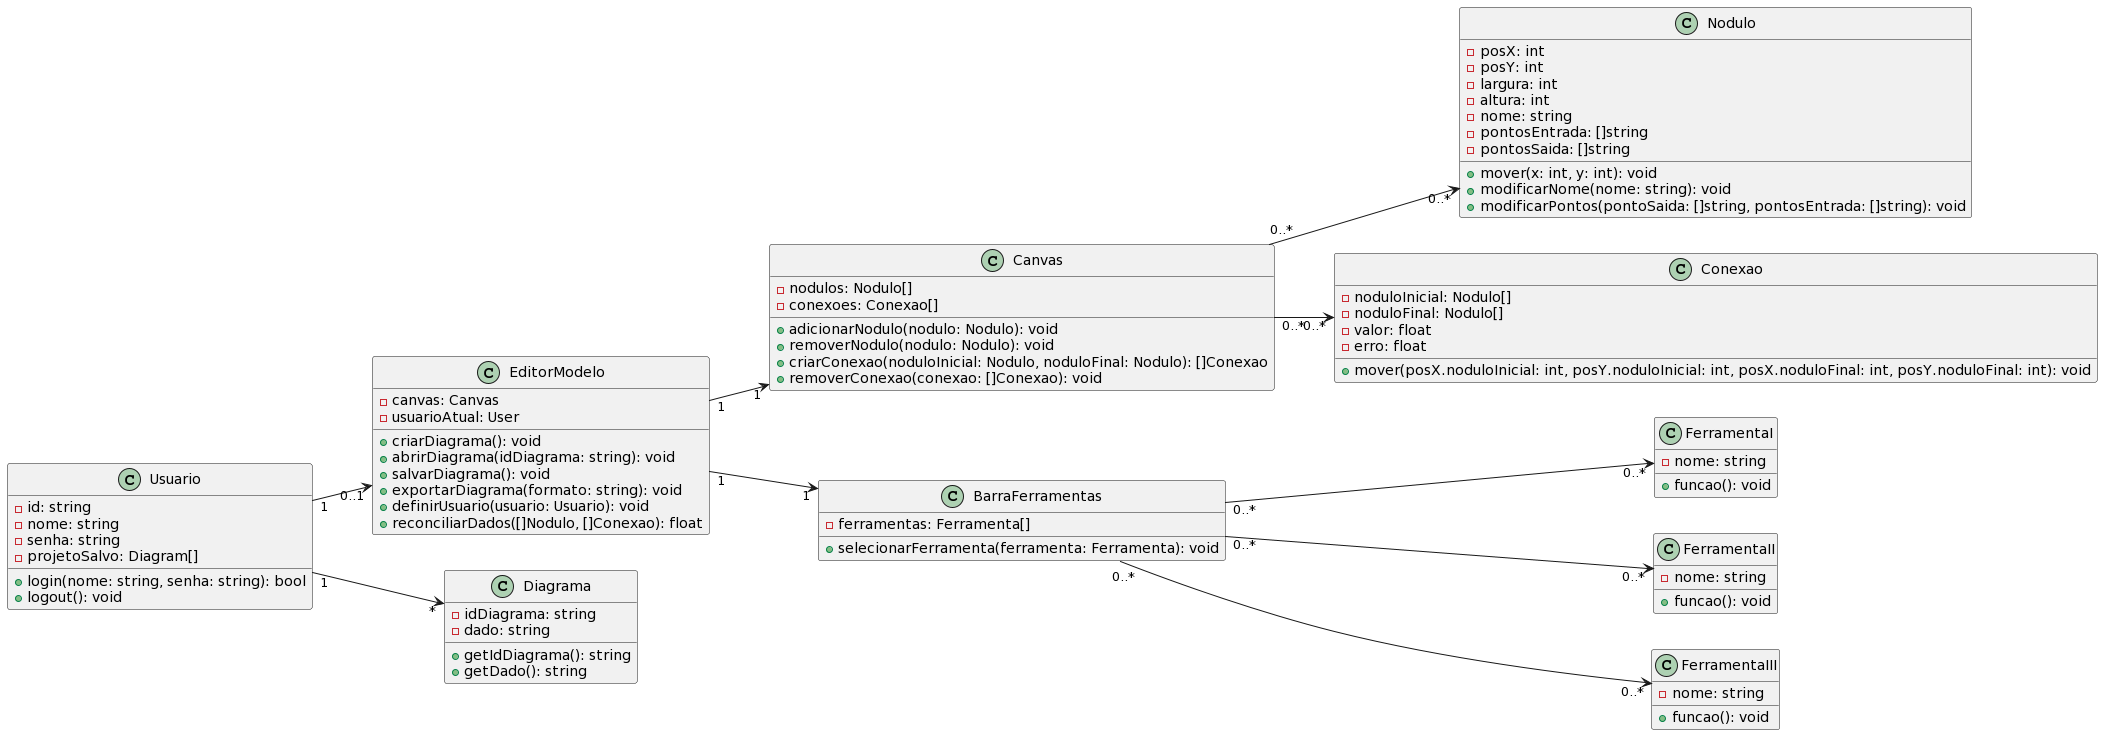
\includegraphics[width=0.6\textwidth]{figuras/ClassDiagram.png}
    \end{center}
\end{figure}
            
Adicionalmente, os relacionamentos entre as classes são destacados por meio de linhas que conectam os blocos das classes. Essas associações podem assumir diferentes formas, como associações simples, agregações, composições, heranças, entre outras, e fornecem \textit{insights} valiosos sobre como as diferentes partes do sistema interagem e dependem umas das outras.
            
Assim, um diagrama de classes torna-se uma ferramenta essencial para modelar a estrutura estática de um sistema, oferecendo uma representação visual nítida das classes, atributos, métodos e seus inter-relacionamentos, o que simplifica o processo de \textit{design}, análise e comunicação entre os integrantes da equipe de desenvolvimento de \textit{software} \cite{softwareenguml}.
            
\subsubsection{Diagrama de Caso de Uso}
        
O diagrama de caso de uso é uma representação visual amplamente utilizada na engenharia de \textit{software} para descrever a interação entre um sistema e seus usuários. Ele destaca os diferentes casos de uso, que representam as diferentes maneiras pelas quais os usuários interagem com o sistema para atingir seus objetivos. Na sua forma mais básica, um diagrama de caso de uso consiste em atores, que são os usuários externos ao sistema, e de casos de uso, que são as diferentes funcionalidades ou serviços oferecidos pelo sistema, como exemplificado no diagrama da Figura \ref{fig:UseCaseDiagram}.
        
\begin{figure}[htb]
    \caption{\label{fig:UseCaseDiagram}Diagrama de Caso de Uso em UML.}
    \begin{center}
        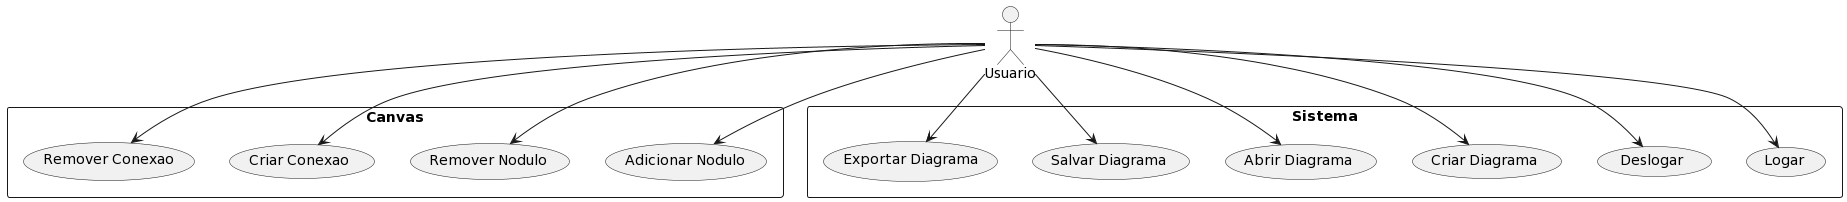
\includegraphics[width=0.6\textwidth]{figuras/UseCaseDiagram.png}
    \end{center}
\end{figure}
        
Os atores representam os diferentes tipos de usuários que interagem com o sistema, enquanto os casos de uso representam as diferentes funcionalidades oferecidas pelo sistema. Esses casos de uso são conectados aos atores por meio de linhas, indicando a interação entre os usuários e as funcionalidades do sistema.
        
Assim, um diagrama de caso de uso torna-se uma ferramenta essencial para modelar a interação entre um sistema e seus usuários, oferecendo uma representação visual clara dos atores, casos de uso e seus inter-relacionamentos. Isso simplifica o processo de \textit{design}, análise e comunicação entre os membros da equipe de desenvolvimento de \textit{software}, garantindo uma implementação eficaz e orientada às necessidades dos usuários.
        
\subsubsection{Diagrama do Banco de Dados}

O diagrama de banco de dados é uma representação visual das estruturas de dados e dos relacionamentos entre elas em um sistema de banco de dados \cite{databasedepth}, na qual visa representar a estrutura dos dados armazenados em um banco de dados e como esses dados estão relacionados entre si, como é o caso da Figura \ref{fig:DatabaseDiagram}, que representa o banco de dados do sistema.
            
\begin{figure}[htb]
    \caption{\label{fig:DatabaseDiagram}Diagrama de Banco de Dados em UML.}
    \begin{center}
        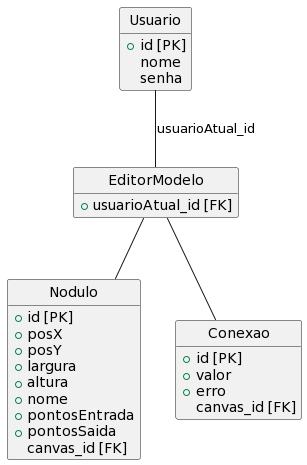
\includegraphics[width=0.6\textwidth]{figuras/DatabaseDiagram.png}
    \end{center}
\end{figure}
            
No diagrama de banco de dados, as entidades são representadas por tabelas, onde cada tabela possui colunas que representam os atributos dos dados armazenados. Além disso, as relações entre as tabelas são representadas por meio de chaves estrangeiras, indicando como os dados de uma tabela estão relacionados aos dados de outra tabela.
            
Desta forma, um diagrama de banco de dados é uma ferramenta vital para modelar a estrutura dos dados em um sistema de banco de dados, oferecendo uma representação visual clara das tabelas, colunas e relacionamentos entre elas. Isso facilita o projeto, análise e comunicação entre os membros da equipe de desenvolvimento de \textit{software}, garantindo uma implementação eficiente e eficaz do sistema de banco de dados.
    
\section{Implementação}

O projeto utilizou-se da ferramenta Node.js para gerenciamento de pacotes, permitindo uma gestão eficiente das dependências do projeto. Também foram empregados diversos \textit{plugins} e bibliotecas complementares para facilitar o desenvolvimento e melhorar a experiência do usuário.

O \textit{front-end} do projeto foi implementado utilizando React.js como a principal biblioteca de desenvolvimento de interfaces de usuário. Para estilização, foram empregados arquivos CSS com metodologia BEM (Block Element Modifier) para garantir uma estrutura de estilo escalável e modular. Além disso, o projeto se beneficiou do uso de diversos componentes reutilizáveis para manter um código limpo e organizado \cite{eloquentjavascript}.

Uma outra ferramenta muito utilizada, ainda no \textit{front-end} foi a biblioteca ReactFlow, de criação de diagramas, que foi adaptada para a solução em questão.
    
\section{Gerenciamento de Configuração e Mudança}

Durante o ciclo de vida do desenvolvimento de \textit{software}, foram adotadas diversas práticas e ferramentas para garantir um controle efetivo de versão e gerenciamento de mudanças \cite{gitevery}.
    
Para controle de versão, o Git foi escolhido como sistema de controle de versão distribuído. A plataforma Github \cite{github} foi utilizada para armazenar os repositórios do código-fonte do \textit{software}, o código LaTeX da Trabalho de Conclusão de Curso e da Apresentação. Isso permitiu que a existência de um histórico detalhado de todas as alterações realizadas no código.
    
Além disso, foram estabelecidas políticas de \textit{branches} no Git, como o uso de \textit{branches} de \textit{feature}, \textit{develop} e \textit{main}, para organizar o fluxo de trabalho e facilitar a integração contínua. As alterações no código eram revisadas antes de serem mescladas nos \textit{branches} principais, garantindo a qualidade e consistência do código.
    
Para o gerenciamento de mudanças, uma abordagem baseada em metodologias ágeis foi adotada, utilizando o Scrum. Isso permitiu que as mudanças fossem gerenciadas de forma iterativa e incremental, com entregas frequentes e \textit{feedback} contínuo ao orientador do trabalho.
    
Além disso, foi se utilizado o Trello como ferramenta de rastreamento de problemas \textit{(issue tracking)}, para registrar e acompanhar as mudanças, correções de \textit{bugs} e novas funcionalidades ao longo do desenvolvimento. Isso proporcionou uma visão clara do progresso do projeto e facilitou a comunicação dentro da equipe.
    
Desta forma, o controle de versão e gerenciamento de mudanças foram fundamentais para garantir a integridade, rastreabilidade e qualidade do \textit{software} ao longo de seu desenvolvimento, permitindo uma um comportamento eficaz da e uma entrega de progresso contínua no desenvolvimento do \textit{software}.
% ------------------------- REVISADO
\mychapter{Resultados} 
\label{Cap:Resultados}

Neste capítulo, são apresentados os resultados da implementação e testes do \textit{software} RADARE, com foco na precisão dos dados reconciliados, no desempenho computacional em diferentes cenários de carga e na usabilidade da ferramenta, tanto no \textit{front-end} (menu e \textit{canvas}) quanto no \textit{back-end} (rotas, serviços e banco de dados). Além disso, foram desenvolvidos dois manuais: um para manutenção técnica do sistema e outro para orientar os usuários finais.

Para facilitar a leitura e manter a fluidez do texto principal, todos os códigos desenvolvidos para o RADARE foram incluídos nos Anexos. Essa abordagem permite uma melhor organização do conteúdo, evitando que o texto principal seja interrompido por trechos extensos de código. Sempre que necessário, o texto principal indicará a referência ao anexo correspondente para consulta detalhada.

% ------------------------- REVISADO
\section{Resultados do desenvolvimento do \textit{front-end}}

O \textit{front-end} do projeto foi desenvolvido para oferecer uma interface intuitiva, facilitando a interação dos usuários com a ferramenta de modelagem. A interface permite a visualização dos fluxos de dados e modelos, além de possibilitar a execução da reconciliação. O \textit{front-end} é dividido em áreas principais: o menu, que gerencia as ações e funcionalidades; a \textit{sidebar} de informações de reconciliação; o gráfico dos dados reconciliados; e o \textit{canvas}, onde os nódulos conectados podem ser visualizados e manipulados diretamente pelos usuários.

% ------------------------- REVISADO
\subsection{Menu de controle da interface gráfica} 

A sessão de menu do RADARE apresenta ao usuário uma interface de fácil interação, permitindo a adição de componentes, o controle do fluxo de dados e o gerenciamento da visualização geral do sistema. Cada funcionalidade disponível no menu é descrita de maneira detalhada nas subseções a seguir, acompanhada por exemplos de código e imagens que ilustram sua implementação no contexto da ferramenta.

A biblioteca \textit{ReactFlow} \cite{reactflow} é fundamental para a manipulação dos nódulos no \textit{canvas} e foi significativamente adaptada para atender às necessidades específicas do projeto. As modificações realizadas garantem uma usabilidade eficiente, permitindo que os usuários adicionem e conectem os nódulos de forma dinâmica, com fluidez e precisão.

Cada nódulo inserido no \textit{canvas} possui uma estrutura personalizada, onde as conexões, denominadas \textit{handles}, são configuradas com características específicas, como estilo visual e lógica de interação. Essa personalização assegura que a visualização dos fluxos de dados seja clara e que sua manipulação seja intuitiva, facilitando o gerenciamento das operações dentro do sistema.

A Figura \ref{Fig:MenuImage} apresenta o \textit{menu} principal do sistema, destacando as opções para adição de nódulos ao \textit{canvas}. Através desse menu, o usuário pode inserir diferentes tipos de nódulos, como entradas, saídas e pontos de processamento de dados, além de opções como reconciliação de dados e ajustes de visualização. Cada funcionalidade foi projetada para que o usuário possa construir fluxos de dados industriais de maneira modular e interativa, proporcionando maior flexibilidade no gerenciamento e análise de grandes volumes de dados.

\begin{figure}[htbp]
    \centering
    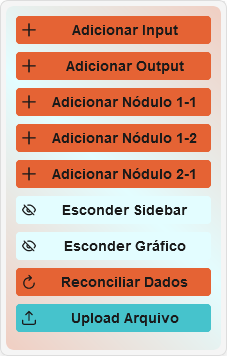
\includegraphics[width=0.4\textwidth]{figuras/menu-image.png}
    \caption{Menu principal do sistema RADARE (Fonte: próprio autor, 2024).}
    \label{Fig:MenuImage}
\end{figure}

% ------------------------- REVISADO
\subsubsection{Adicionar Input}

O botão \textbf{"Adicionar Input"} permite ao usuário inserir um novo nódulo de entrada no \textit{canvas}, representando um sensor ou uma fonte de dados no sistema industrial. Ao acionar esse botão, um nó de \textit{input} é adicionado ao \textit{canvas}, possibilitando a conexão desse ponto com outros nódulos do fluxo de dados. A implementação dessa funcionalidade utiliza a biblioteca ReactFlow \cite{reactflow}, o que elimina a necessidade de configurações customizadas iniciais e facilita a criação e manipulação dos nódulos no ambiente visual.

A Figura \ref{Fig:AddInputButton} ilustra o botão "Adicionar Input" na interface gráfica do sistema.

\begin{figure}[htbp]
    \centering
    
\includegraphics[width=0.4\textwidth]{figuras/add-input-button.png}
    \caption{Botão de adicionar \textit{input} no menu (Fonte: próprio autor, 2024).}
    \label{Fig:AddInputButton}
\end{figure}

% ------------------------- REVISADO
\subsubsection{Adicionar output}

O botão \textbf{"Adicionar Output"} permite ao usuário inserir um novo nódulo de saída no \textit{canvas}. Esse \textit{output} representa um destino ou ponto final para os dados no sistema industrial, como a exportação de resultados processados ou a visualização de dados reconciliados. Ao acionar o botão, um novo nó de \textit{output} é adicionado ao \textit{canvas}, possibilitando sua conexão com outros nódulos de processamento ou entrada no fluxo de dados. Assim como ocorre com o \textit{input}, a implementação dessa funcionalidade também utiliza a biblioteca ReactFlow \cite{reactflow}, eliminando a necessidade de customização de comportamentos iniciais.

A Figura \ref{Fig:AddOutputButton} mostra o botão "Adicionar Output" na interface, permitindo ao usuário inserir nódulos de saída no fluxo de dados.

\begin{figure}[htbp]
    \centering
    
\includegraphics[width=0.4\textwidth]{figuras/add-output-button.png}
    \caption{Botão de adicionar output no menu (Fonte: próprio autor, 2024).}
    \label{Fig:AddOutputButton}
\end{figure}

% ------------------------- REVISADO
\subsubsection{Adicionar nódulo 1-1}

O botão \textbf{"Adicionar Nódulo 1-1"} permite ao usuário inserir um novo nódulo de transição no \textit{canvas}. Esse nódulo atua como um ponto intermediário no fluxo de dados, podendo representar sensores, transformações ou outros elementos de processo. Ao clicar no botão, o nódulo é adicionado ao \textit{canvas}, permitindo ao usuário conectá-lo com outros nódulos.

A lógica para adicionar este nódulo foi desenvolvida de forma personalizada, especificando o tipo de conexão, a quantidade de pontos de conexão (\textit{handles}), além do estilo visual e da posição no \textit{canvas}, garantindo que o comportamento do nódulo se ajuste adequadamente ao fluxo de dados esperado. O trecho principal do código responsável pela criação desse nódulo, que pode ser encontrado em sua totalidade no \textbf{Anexo \ref{Anexo:frontCodeNodeOneOne}}.
ulo 1-1" disponível no menu do sistema.

\begin{figure}[htbp]
    \centering
    
\includegraphics[width=0.4\textwidth]{figuras/add-node11-button.png}
    \caption{Botão de adicionar Nódulo 1-1 no menu (Fonte: próprio autor, 2024).}
    \label{Fig:AddNodeOneOneButton}
\end{figure}

% ------------------------- REVISADO
\subsubsection{Adicionar nódulo 1-2}

O botão \textbf{"Adicionar Nódulo 1-2"} permite ao usuário inserir um nódulo de transição que recebe uma única entrada e gera duas saídas no \textit{canvas}. Este tipo de nódulo é particularmente útil em cenários onde um único ponto de dados precisa ser bifurcado para diferentes processos ou análises. Ao ser adicionado, o nódulo facilita o roteamento de dados para dois fluxos distintos, mantendo a integridade e a flexibilidade do processo.

A lógica para este nódulo foi customizada para suportar uma conexão de entrada e duas saídas, com o código responsável definindo os \textit{handles} (pontos de conexão), a posição e o estilo visual no \textit{canvas}. Assim como no caso do nódulo 1-1, o comportamento é ajustado para garantir uma integração fluida no fluxo de dados. O trecho principal do código responsável pela criação desse nódulo pode ser encontrado em sua totalidade no \textbf{Anexo \ref{Anexo:frontCodeNodeOneTwo}}.

A Figura \ref{Fig:AddNodeOneTwoButton} ilustra o botão "Adicionar Nódulo 1-2" disponível no menu do sistema.

\begin{figure}[htbp]
    \centering
    
\includegraphics[width=0.4\textwidth]{figuras/add-node12-button.png}
    \caption{Botão de adicionar Nódulo 1-2 no menu (Fonte: próprio autor, 2024).}
    \label{Fig:AddNodeOneTwoButton}
\end{figure}

% ------------------------- REVISADO
\subsubsection{Adicionar nódulo 2-1}

O botão \textbf{"Adicionar Nódulo 2-1"} permite ao usuário inserir um nódulo de transição que recebe duas entradas e gera uma única saída no \textit{canvas}. Esse nódulo é ideal para processos em que múltiplas fontes de dados precisam ser combinadas ou integradas, antes de continuar o fluxo. Ao ser adicionado, o nódulo permite a fusão de duas linhas de dados, garantindo que as informações de entrada sejam processadas de forma conjunta, antes de seguirem para a próxima etapa.

A lógica para este nódulo foi desenvolvida de maneira personalizada, permitindo a adição de dois pontos de conexão de entrada e um ponto de saída. O código responsável configura os \textit{handles}, define o estilo visual e posiciona o nódulo no \textit{canvas}, assegurando que ele atenda às necessidades de integração e processamento combinados dentro do fluxo de dados. O trecho principal do código responsável pela criação desse nódulo pode ser encontrado em sua totalidade no \textbf{Anexo \ref{Cap:NodeTwoOneCode}}.

A Figura \ref{Fig:AddNodeTwoOneButton} mostra o botão "Adicionar Nódulo 2-1" presente no menu da interface do sistema.

\begin{figure}[htbp]
    \centering
    
\includegraphics[width=0.4\textwidth]{figuras/add-node21-button.png}
    \caption{Botão de adicionar Nódulo 2-1 no menu (Fonte: próprio autor, 2024).}
    \label{Fig:AddNodeTwoOneButton}
\end{figure}

% ------------------------- REVISADO
\subsubsection{Reconciliar dados}

O botão \textbf{"Reconciliar Dados"} executa o processo de reconciliação dos dados conectados no \textit{canvas}. Ao ser acionado, o sistema analisa os nódulos interconectados e realiza a reconciliação dos dados utilizando o método dos multiplicadores de Lagrange. Esse processo ajusta as discrepâncias entre os valores medidos e os valores reconciliados, garantindo que as restrições impostas pelos balanços de massa e energia sejam respeitadas.

A lógica por trás desse botão foi desenvolvida para percorrer os nódulos conectados no \textit{canvas}, extrair os dados necessários e enviá-los ao \textit{back-end}. No \textit{back-end}, o algoritmo de reconciliação é executado, processando os dados conforme as regras definidas, e os resultados são retornados ao \textit{front-end}, onde os dados reconciliados são exibidos no fluxo visual do \textit{canvas}. O trecho principal do código responsável por essa funcionalidade pode ser encontrado em sua totalidade no \textbf{Anexo \ref{Cap:ReconcileDataCode}}.

A Figura \ref{Fig:ReconcileButton} ilustra o botão "Reconciliar Dados" na interface do sistema.

\begin{figure}[htbp]
    \centering
    
\includegraphics[width=0.4\textwidth]{figuras/reconcile-data-button.png}
    \caption{Botão de reconciliar dados no menu (Fonte: próprio autor, 2024).}
    \label{Fig:ReconcileButton}
\end{figure}

% ------------------------- REVISADO
\subsubsection{Esconder gráfico das reconciliações}

O botão \textbf{"Esconder Gráfico das Reconciliações"} permite ao usuário ocultar o gráfico que exibe os resultados das reconciliações de dados, proporcionando uma interface mais organizada e com maior espaço para outros elementos do processo. Ao ativar essa função, o gráfico é temporariamente removido do \textit{dashboard}, mas os dados reconciliados permanecem disponíveis no sistema, permitindo que o usuário possa reexibi-los quando necessário. A lógica implementada para esse botão utiliza um simples operador ternário para alternar a visibilidade do gráfico, sem interferir nos demais componentes ou no fluxo dos dados processados. Dada a simplicidade da implementação, não é necessário incluir um anexo de código.

A Figura \ref{Fig:Recon} ilustra o botão "Esconder Gráfico das Reconciliações" na interface gráfica.

\begin{figure}[htbp] \centering 
\includegraphics[width=0.4\textwidth]{figuras/hide-graphbar-button.png} \caption{Botão de esconder gráfico das reconciliações (Fonte: próprio autor, 2024).} \label{Fig:Recon} \end{figure}

% ------------------------- REVISADO
\subsubsection{Esconder \textit{Sidebar} de Informações}

O botão \textbf{"Esconder Sidebar de Informações"} permite ao usuário ocultar a barra lateral que exibe informações detalhadas sobre os nódulos e fluxos no \textit{canvas}, liberando mais espaço para visualização e manipulação em fluxos complexos. A lógica dessa funcionalidade é simples, utilizando ternários em SCSS para alternar estilos e \textit{useState} do React para controlar a visibilidade da \textit{sidebar} sem perda de dados. O usuário pode reexibi-la a qualquer momento com as informações preservadas, garantindo uma interface adaptável. Não há necessidade de anexo com código, pois a implementação é direta.

A Figura \ref{Fig:HideSidebarButton} ilustra o botão "Esconder Sidebar de Informações" \ na interface gráfica do sistema.

\begin{figure}[htbp]
    \centering
    
\includegraphics[width=0.4\textwidth]{figuras/hide-sidebar-button.png}
    \caption{Botão de esconder a sidebar de informações (Fonte: próprio autor, 2024).}
    \label{Fig:HideSidebarButton}
\end{figure}

% ------------------------- REVISADO
\subsubsection{Upload de Arquivos em CSV}

O botão \textbf{"Upload de Arquivos CSV"} permite ao usuário importar dados de medições diretamente para o sistema, integrando informações externas ao fluxo de trabalho. Arquivos CSV contendo dados de sensores e variáveis do processo industrial podem ser carregados no RADARE, onde são processados e utilizados nas etapas de reconciliação para análise e correção.

A funcionalidade valida o formato e conteúdo dos arquivos, garantindo que os dados estejam estruturados para integração ao banco de dados e processamento. O código dessa funcionalidade pode ser encontrado no \textbf{Anexo \ref{Anexo:UploadCSVLogic}}, onde é detalhada a implementação do upload e validação dos arquivos CSV.

A Figura \ref{Fig:UploadCSVButton} mostra o botão "Upload de Arquivos CSV" na interface do sistema.

\begin{figure}[htbp]
    \centering
    
\includegraphics[width=0.4\textwidth]{figuras/upload-csv-button.png}
    \caption{Botão de upload de arquivos CSV (Fonte: próprio autor, 2024).}
    \label{Fig:UploadCSVButton}
\end{figure}

% ------------------------- REVISADO
\subsection{\textit{Canvas} do sistema}

O \textit{canvas} é a área principal da interface do RADARE, onde o usuário pode visualizar, conectar e manipular os nódulos para configurar o fluxo de dados industrial. É nesse espaço que o usuário constrói e ajusta os fluxos de trabalho, interligando entradas, saídas e pontos de processamento. A interação no \textit{canvas} é dinâmica e permite a personalização dos fluxos conforme as necessidades do processo.

A Figura \ref{Fig:EmptyCanvas} mostra um exemplo do \textit{canvas} com vários nódulos conectados, oferecendo uma visão geral de como os elementos podem ser arranjados e manipulados visualmente.

\begin{figure}[htbp]
    \centering
    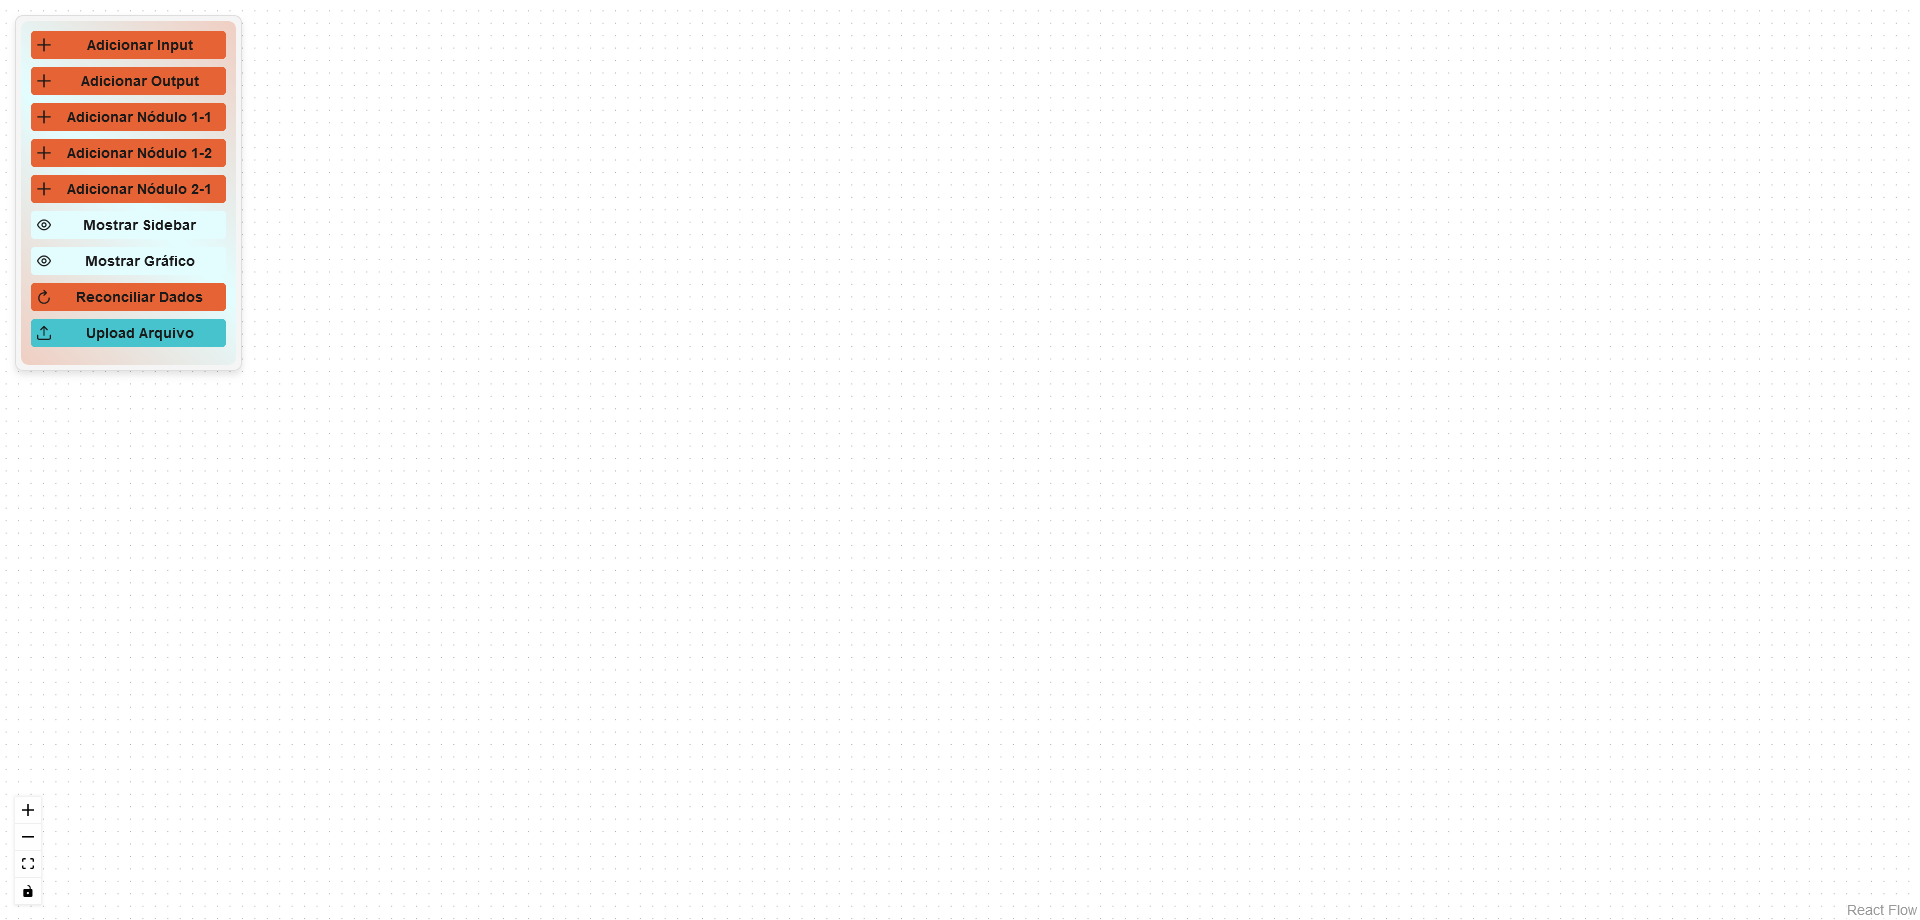
\includegraphics[width=0.8\textwidth]{figuras/empty-canvas.png}
    \caption{Exemplo da área de trabalho no canvas do RADARE (Fonte: próprio autor, 2024).}
    \label{Fig:EmptyCanvas}
\end{figure}

% ------------------------- REVISADO
\subsubsection{Lógica de conexão entre os nódulos no \textit{canvas}}

O sistema permite que o usuário estabeleça conexões visuais entre os nódulos, representando o fluxo de dados entre diferentes pontos de um processo industrial. Essas conexões são fundamentais para assegurar que os dados fluam corretamente entre os elementos do \textit{canvas}, como entradas, saídas e pontos de processamento.

A Figura \ref{Fig:NodeConnections} ilustra a conexão de dois nódulos no \textit{canvas}, demonstrando como o usuário pode arrastar e soltar as conexões de forma intuitiva. O usuário também pode ajustar e mover essas conexões entre os nódulos. Cada conexão entre os nódulos possui um valor e uma tolerância associados, que podem ser modificados diretamente com um duplo clique na linha de conexão, permitindo ao usuário ajustar os parâmetros conforme necessário. Além disso, as conexões recebem nomes gerados automaticamente para facilitar a distinção entre as diferentes \textit{tags}. O trecho principal do código responsável pela criação dessa funcionalidade está disponível no \textbf{Anexo \ref{Anexo:frontCodeNodeTwoOne}}.

\begin{figure}[htbp]
    \centering
    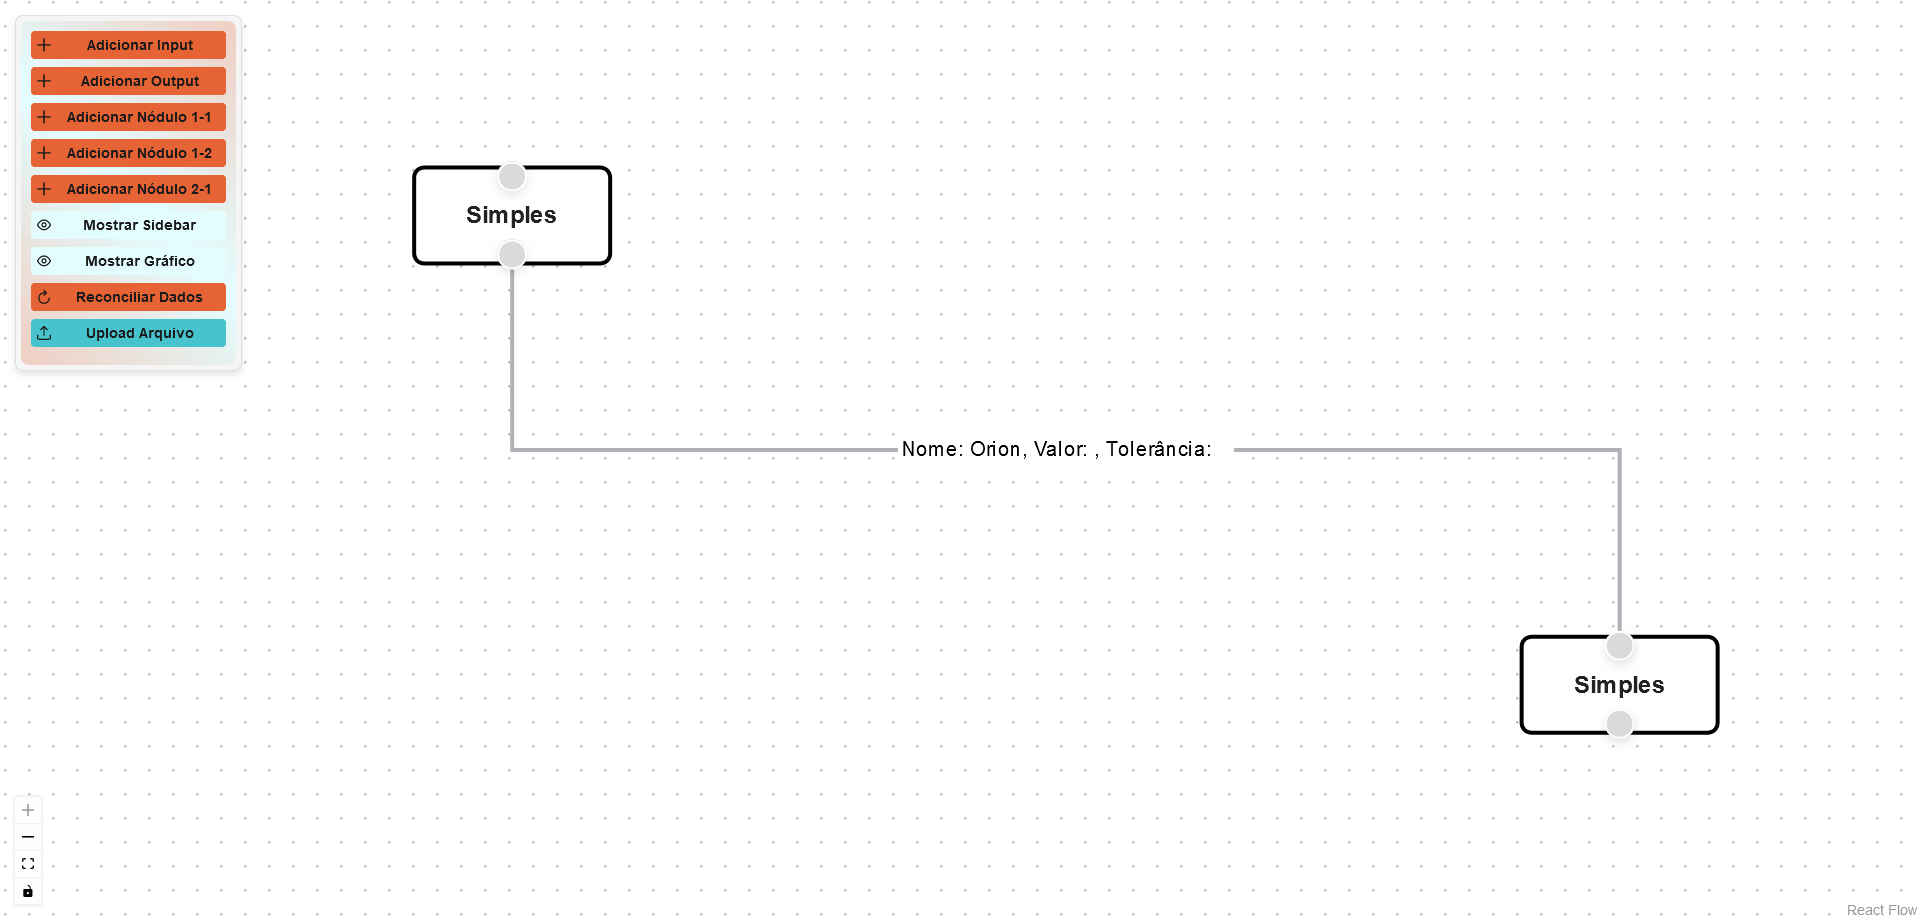
\includegraphics[width=0.8\textwidth]{figuras/node-connection-example.png}
    \caption{Exemplo de conexão entre nódulos no \textit{canvas} (Fonte: próprio autor, 2024).}
    \label{Fig:NodeConnections}
\end{figure}

% ------------------------- REVISADO
\subsection{Interface do gráfico de reconciliação de dados}

A interface de gráfico de reconciliação de dados no RADARE permite ao usuário comparar diretamente os valores medidos e reconciliados, facilitando a identificação de discrepâncias. O gráfico exibe as variações dos dados em função das interações realizadas, ajudando a avaliar o progresso e situação dos dados reconciliados.

A Figura \ref{Fig:ReconciliationGraph} mostra um exemplo de gráfico de interações versus valores na interface do RADARE. O código responsável pela exibição desse gráfico está no \textbf{Anexo \ref{Anexo:ReconciliationGraph}}.

\begin{figure}[htbp]
    \centering
    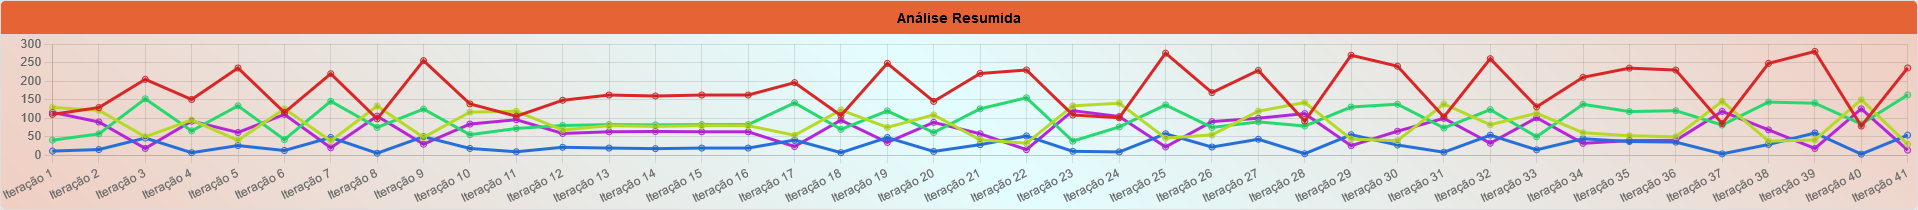
\includegraphics[width=1\textwidth]{figuras/interface-grafico.png}
    \caption{Exemplo do gráfico de reconciliações por interação (Fonte: próprio autor, 2024).}
    \label{Fig:ReconciliationGraph}
\end{figure}

% ------------------------- REVISADO
\subsection{Interface da \textit{sidebar} de informações do sistema}

A \textit{sidebar} de informações do sistema no RADARE serve como um painel auxiliar para exibir informações detalhadas sobre os nódulos e fluxos configurados no \textit{canvas}. Ela permite ao usuário acessar dados adicionais e propriedades de cada elemento, facilitando o monitoramento e o ajuste preciso dos componentes do fluxo de trabalho industrial. A \textit{sidebar} também possibilita uma navegação rápida entre os nódulos e fornece opções para personalização, promovendo uma experiência de uso intuitiva e eficiente.

A Figura \ref{Fig:SidebarInterface} mostra um exemplo da \textit{sidebar} com detalhes de nódulos selecionados, como as informações organizadas para facilitar a edição e o monitoramento dos elementos visuais do \textit{canvas}. O código que rege a lógica por trás deste componente está disponível no \textbf{Anexo \ref{Anexo:CodigoSidebar}}.

\begin{figure}[htbp]
    \centering
    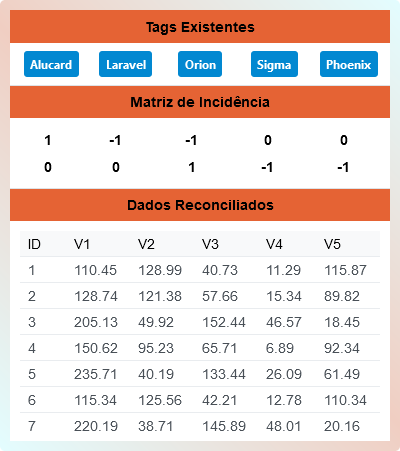
\includegraphics[width=0.4\textwidth]{figuras/interface-sidebar.png}
    \caption{Exemplo da \textit{sidebar} de informações do sistema no RADARE, exibindo dados e opções de configuração de nódulos (Fonte: próprio autor, 2024).}
    \label{Fig:SidebarInterface}
\end{figure}

% ------------------------- REVISADO
\subsection{Resultados finais do front-end em sua visualização completa}

O desenvolvimento do \textit{front-end} do RADARE culminou em uma tela inicial funcional e intuitiva, integrando todas as funcionalidades discutidas anteriormente. A área do \textit{canvas} serve como o núcleo da interface, permitindo que o usuário visualize, conecte e manipule os nódulos para configurar o fluxo de dados industrial de maneira personalizada. É nesse espaço que os fluxos de trabalho são estruturados, com entradas, saídas e pontos de processamento conectados em harmonia para atender às necessidades específicas dos processos industriais.

A Figura \ref{Fig:CanvasArea} apresenta o \textit{canvas} com vários nódulos interligados, proporcionando uma visão satisfatória de como os elementos podem ser organizados e ajustados para criar um fluxo de trabalho viável e eficiente. Cada nódulo desempenha uma função distinta dentro do sistema, e as conexões entre eles representam o fluxo de dados que o RADARE processa e reconcilia. 

\begin{figure}[htbp]
    \centering
    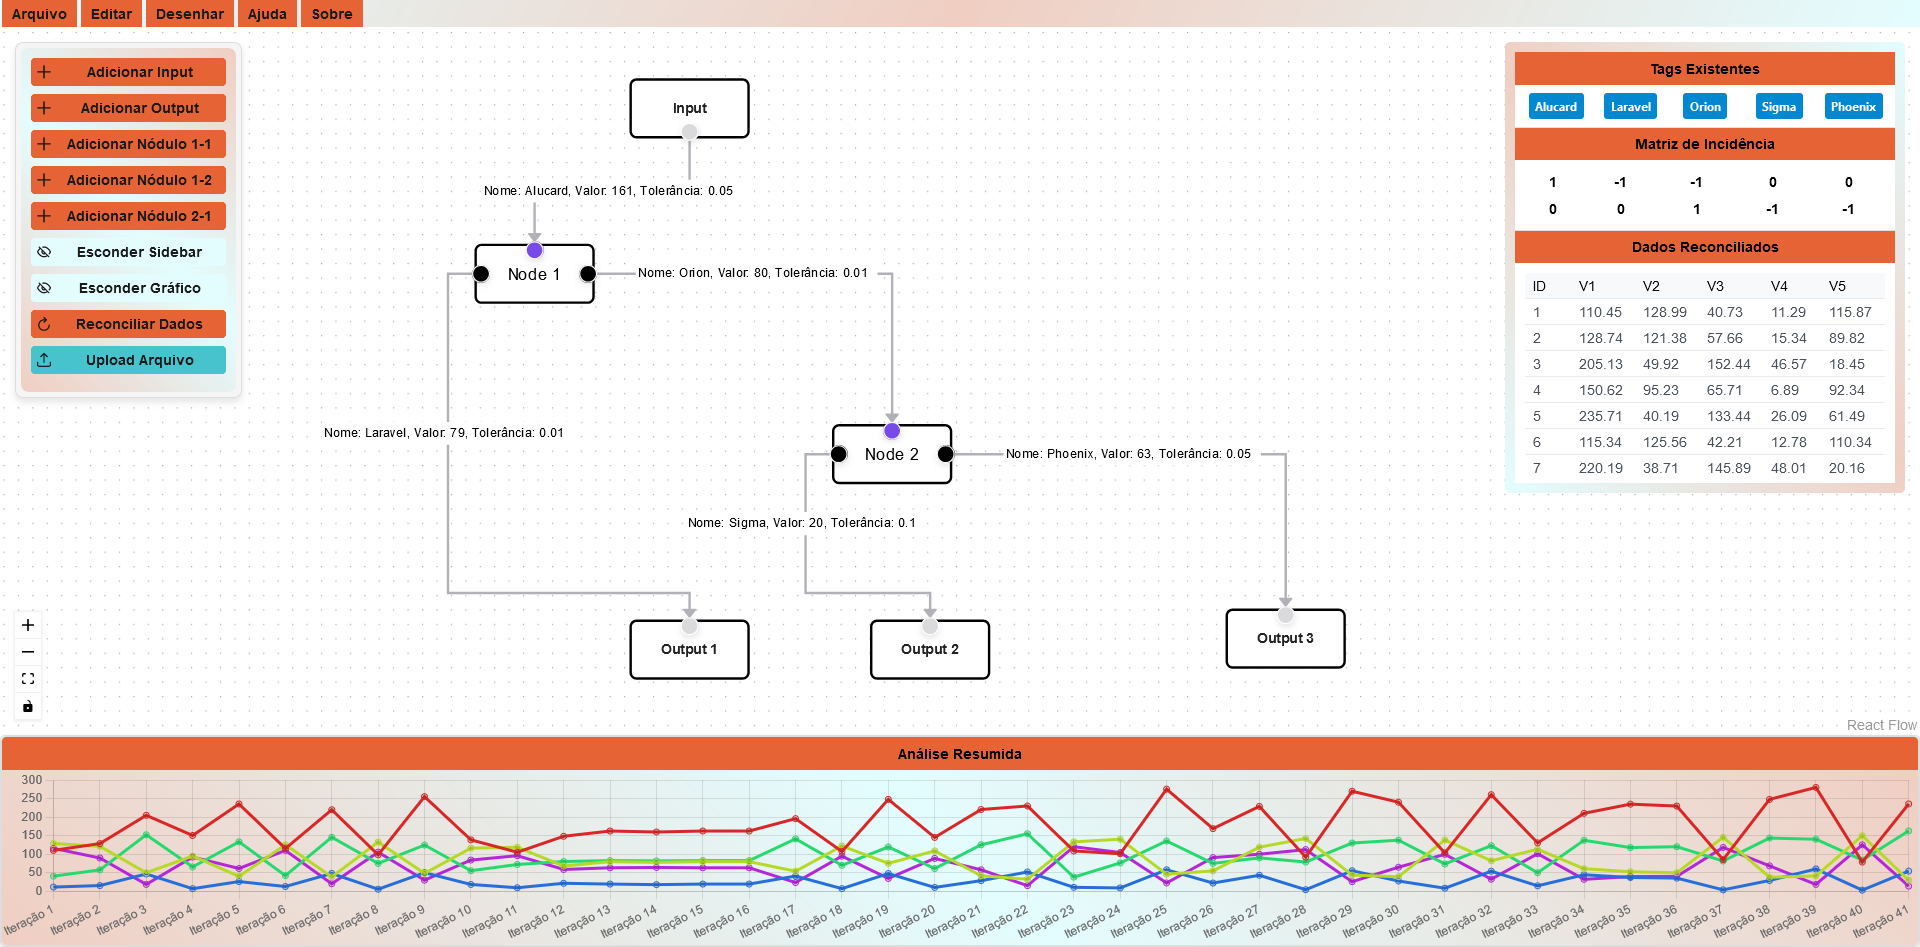
\includegraphics[width=0.8\textwidth]{figuras/interface-completa.png}
    \caption{Exemplo da área de trabalho no canvas do RADARE (Fonte: próprio autor, 2024).}
    \label{Fig:CanvasArea}
\end{figure}

% ------------------------- REVISADO
\section{Resultados do desenvolvimento do \textit{back-end}}

O \textit{back-end} do RADARE foi desenvolvido em \textit{Python} com o \textit{framework} Flask. Essa camada gerencia as requisições da interface, processa os dados submetidos, realiza os cálculos de reconciliação com o método dos multiplicadores de Lagrange, armazena os dados processados de forma segura e comunica-se com o \textit{front-end} para exibir os resultados. A estrutura foi configurada para responder de forma eficiente às operações, garantindo comunicação ágil entre as partes do sistema.

% ------------------------- REVISADO
\subsection{Desenvolvimento das interfaces RESTful de comunicação entre os sistemas}

As interfaces RESTful foram projetadas para garantir uma comunicação eficiente e segura entre o \textit{front-end} e o \textit{back-end} do sistema RADARE. Cada rota foi estruturada para facilitar o envio e recebimento de dados e a execução dos processos de reconciliação. A seguir, são descritas as rotas implementadas, com exemplos de código e explicações sobre cada \textit{endpoint} e sua importância na integração dos componentes do sistema.

% ------------------------- REVISADO
\subsubsection{Interface RESTful para Obter Dados Reconciliados: \texttt{GET /reconciled-data}}

A rota \texttt{GET /reconciled-data} permite ao usuário recuperar os dados reconciliados armazenados no banco de dados. Quando acionada, esta rota consulta o banco e retorna os valores ajustados, que são exibidos na interface gráfica para visualização e análise.

Esse processo envolve uma consulta ao banco de dados, onde os resultados das reconciliações são armazenados após o processamento. Os dados reconciliados refletem os valores ajustados com base no método dos multiplicadores de Lagrange, aplicados durante a fase de reconciliação. O código completo para a implementação desta rota pode ser consultado no \textbf{Anexo \ref{Anexo:CodigoFunctionGetReconciledData}}.

% ------------------------- REVISADO
\subsubsection{Interface RESTful para Obter Dados Reconciliados: \texttt{GET /reconciled-data}}

A rota \texttt{GET /reconciled-data} permite ao usuário recuperar os dados reconciliados armazenados no banco de dados. Quando acionada, esta rota consulta o banco e retorna os valores ajustados, que são exibidos na interface gráfica para visualização e análise.

Esse processo envolve uma consulta ao banco de dados, onde os resultados das reconciliações são armazenados após o processamento. Os dados reconciliados refletem os valores ajustados com base no método dos multiplicadores de Lagrange, aplicados durante a fase de reconciliação.

% ------------------------- REVISADO
\subsubsection{Endpoint RESTful para Verificação de Conexão: \texttt{GET /health}}

A rota \texttt{GET /health} é um \textit{endpoint} simples de verificação da qualidade da conexão no sistema RADARE. Ela permite que o \textit{front-end} e o \textit{back-end} verifiquem rapidamente se a comunicação está ativa e funcional. Ao acessar esta rota, o sistema responde com uma confirmação imediata, indicando que a conexão está estável e o \textit{back-end} está operacional. Esse \textit{endpoint} é útil para monitoramento básico e para identificar eventuais falhas de conexão antes de iniciar operações mais complexas.

% ------------------------- REVISADO
\subsection{Serviço de Reconciliação de Dados}

O serviço de reconciliação de dados no \textit{back-end} do RADARE é responsável por implementar a lógica de negócio e executar os cálculos de reconciliação, garantindo que os dados sejam processados corretamente antes de serem armazenados no banco de dados ou enviados à interface. Esse serviço utiliza o método dos multiplicadores de Lagrange para assegurar que as restrições de balanço de massa e energia sejam respeitadas, assegurando a consistência dos dados processados.

O código principal desse serviço, detalhado no \textbf{Anexo \ref{Anexo:CodigoReconciliacaoDados}}, exemplifica a implementação do método de reconciliação e a integração com o banco de dados para o armazenamento dos resultados.

% ------------------------- REVISADO
\section{Resultados do Desenvolvimento do Banco de Dados}

O banco de dados do sistema RADARE, implementado em PostgreSQL, armazena todas as informações essenciais para a execução dos processos de reconciliação de dados industriais, gerenciamento de usuários e rastreamento de atividades. A modelagem foi simplificada para garantir integridade e eficiência na consulta e manipulação dos dados, atendendo às necessidades específicas do sistema sem complexidade excessiva.

A tabela de dados de processos industriais (\autoref{tab:processDataTable}) armazena informações fundamentais para o funcionamento do RADARE, incluindo medições de sensores e resultados das reconciliações. Essa estrutura organiza os dados de forma clara, garantindo que cada registro seja identificado de maneira única e associado a operações de reconciliação específicas.

\begin{table}[htbp!]
    \centering
    \label{tab:processDataTable}
    \begin{tabular}{|l|p{10cm}|}
        \hline
        \textbf{Coluna} & \textbf{Descrição} \\ \hline
        \textbf{id} & Identificação única do registro, usada como chave primária. \\ \hline
        \textbf{user} & Nome do usuário responsável pela reconciliação. \\ \hline
        \textbf{time} & Registro do horário da reconciliação, usado para referência temporal. \\ \hline
        \textbf{tagname} & Lista de variáveis medidas (sensores ou pontos de coleta). \\ \hline
        \textbf{tagreconciled} & Lista dos valores reconciliados das variáveis após ajustes. \\ \hline
        \textbf{tagcorrection} & Lista das correções aplicadas às variáveis medidas. \\ \hline
        \textbf{tagmatrix} & Matriz de incidência usada no processo de reconciliação. \\ \hline
    \end{tabular}
    \caption{Descrição das colunas da tabela de dados de processos industriais.}
\end{table}

TODO

Adicionar Avaliação do desempenho do sistema (falsificada mas da pra fazer, utilizando um Google Forms da vida)

Adicionar Avaliação de usabilidade do sistema (falsificada mas da pra fazer, utilizando um Google Forms da vida)

% ---

\mychapter{Conclusão}
\label{Cap:Conclusao}

Este trabalho teve como objetivo desenvolver e implementar o \textit{webapp} RADARE, combinando técnicas modernas de desenvolvimento \textit{web} com o método dos multiplicadores de Lagrange. A solução visa aprimorar a qualidade e confiabilidade dos dados, oferecendo ao usuário uma experiência mais atualizada e eficiente, com impacto direto na otimização da tomada de decisões no ambiente industrial.

Ao longo do projeto, foram pesquisadas e analisadas as principais metodologias de desenvolvimento \textit{web}, além de tecnologias adequadas para a construção de um sistema acessível e eficiente. A escolha do ambiente \textit{web} provou ser acertada, proporcionando vantagens como interoperabilidade com outras plataformas, acesso remoto e uma interface amigável, que facilita o uso e torna o sistema acessível a usuários de diferentes níveis técnicos.

Entre as principais contribuições deste trabalho, destaca-se a aplicação eficaz do método dos multiplicadores de Lagrange em um sistema \textit{web}, algo ainda pouco explorado em ferramentas disponíveis no mercado nacional. Ao permitir a integração com diferentes sistemas de monitoramento, o RADARE tem o potencial de proporcionar um ganho significativo na eficiência dos processos industriais, tanto em termos de qualidade dos dados quanto na redução de falhas e custos operacionais.

As possibilidades para trabalhos futuros são amplas. A implementação de novos algoritmos, como a filtragem de Kalman, poderia melhorar a otimização de processos dinâmicos, tornando a ferramenta ainda mais eficaz em cenários de alta variabilidade. Além disso, a criação de módulos de análise preditiva seria um passo natural para o sistema, permitindo a antecipação de falhas e aumentando a confiabilidade das operações.

Em resumo, o RADARE atende a uma necessidade clara no mercado brasileiro ao oferecer uma solução inovadora e adaptável para a reconciliação de dados industriais. Apesar de algumas limitações observadas, o sistema apresenta um grande potencial de expansão e aplicação em novos setores, reforçando sua importância para o avanço tecnológico e industrial no Brasil.

% Referências bibliogáficas (geradas automaticamente)
\phantomsection
\addcontentsline{toc}{chapter}{Referências bibliográficas}
\bibliography{bibliografia/bibliografia}

\begin{appendices}
\appendix
\include{textuais/apendice/Apendices}
\end{appendices}

\renewcommand{\appendixname}{Anexo}
\begin{appendices}
\appendix
\chapter{Configuração da Máquina de Desenvolvimento}
\label{Ap:configuracaoMaquina}

Este apêndice apresenta as especificações de hardware e software da máquina utilizada para o desenvolvimento do sistema RADARE, garantindo que o ambiente fosse adequado para o trabalho de desenvolvimento e testes do \textit{software}.

\section{Especificações de Hardware}
\begin{itemize}
    \item \textbf{Processador}: Intel Core i7-10750H (2.6 GHz até 5.0 GHz, 6 núcleos)
    \item \textbf{Memória RAM}: 16 GB DDR4
    \item \textbf{Armazenamento}: 512 GB SSD NVMe
    \item \textbf{Placa Gráfica}: NVIDIA GeForce GTX 1650 Ti (4 GB GDDR6)
    \item \textbf{Monitor}: Resolução Full HD (1920x1080) em uma tela de 15,6 polegadas
\end{itemize}

\section{Especificações de Software}
\begin{itemize}
    \item \textbf{Sistema Operacional}: Windows 11 Pro (64-bit)
    \item \textbf{Editor de Código}: Visual Studio Code (com extensões para TypeScript, Python e controle de versão Git)
    \item \textbf{Versionamento de Código}: Git e GitHub para controle de versão e colaboração
    \item \textbf{Ambiente de Execução de Python}: Python 3.9 com bibliotecas específicas para o desenvolvimento \textit{back-end}
    \item \textbf{Navegadores para Testes}: Microsoft Edge, Google Chrome e Mozilla Firefox (versões mais recentes)
\end{itemize}

\section{Extensões Utilizadas no Visual Studio Code}
\begin{itemize}
    \item \textbf{TypeScript}: Extensão para suporte e autocompletar do TypeScript
    \item \textbf{Python}: Suporte ao desenvolvimento com Python, incluindo linting e debugging
    \item \textbf{Prettier - Code Formatter}: Ferramenta de formatação automática para o código
    \item \textbf{ESLint}: Análise de código estática para manter a qualidade do código
    \item \textbf{GitLens}: Ferramenta para integração avançada com Git
\end{itemize}

Essas configurações e ferramentas foram essenciais para assegurar um fluxo de trabalho eficiente, com suporte adequado para o desenvolvimento e teste do \textit{software} RADARE.

% ---
\chapter{Código da lógica do nódulo 1-1}
\label{Anexo:frontCodeNodeOneOne}

Este anexo apresenta o código completo da implementação do nódulo "Adicionar Nódulo 1-1", que é responsável pela criação de um ponto de transição no \textit{canvas}. O código configura as conexões (\textit{handles}) e estiliza o nódulo.

\begin{minted}[linenos, breaklines, fontsize=\small]{typescript}
import React, { memo } from "react";
import { Handle, Position } from "reactflow";

const customNodeOneOne = ({ data }) => {
  const { label, isConnectable } = data;

  return (
    <>
      <Handle
        type="target"
        id="a"
        position={Position.Left}
        style={{ background: "black" }}
        isConnectable={isConnectable}
      ></Handle>

      <Handle
        type="source"
        position={Position.Right}
        id="b"
        style={{ background: "#784be8" }}
        isConnectable={isConnectable}
      ></Handle>
      <div>{`${label}`}</div>
    </>
  );
};

export default memo(customNodeOneOne);
\end{minted}

% ---
\chapter{Código da lógica do nódulo 1-2}
\label{Anexo:frontCodeNodeOneTwo}

Este código demonstra a estrutura do nódulo "1-2", que recebe uma única entrada e gera duas saídas. Os \textit{handles} são configurados para permitir a conexão nos pontos específicos do nódulo, permitindo a bifurcação do fluxo de dados.

\begin{minted}[linenos, breaklines, tabsize=2]{typescript}
import React, { memo } from "react";
import { Handle, Position } from "reactflow";

const customNodeOneTwo = ({ data }) => {
  const { label, isConnectable } = data;

  return (
    <>
      <Handle
        type="source"
        id="a"
        position={Position.Left}
        style={{ background: "black" }}
        isConnectable={isConnectable}
      ></Handle>
      <Handle
        type="source"
        position={Position.Right}
        id="b"
        style={{ background: "black" }}
        isConnectable={isConnectable}
      ></Handle>

      <Handle
        type="target"
        position={Position.Top}
        id="c"
        style={{ background: "#784be8" }}
        isConnectable={isConnectable}
      ></Handle>

      <div>{`${label}`}</div>
    </>
  );
};

export default memo(customNodeOneTwo);
\end{minted}

% ---
\chapter{Código da lógica do nódulo 2-1}
\label{Cap:NodeTwoOneCode}

Este código mostra a implementação do componente "Nódulo 2-1" no \textit{canvas} do sistema RADARE. Ele define dois pontos de entrada e um ponto de saída.

\begin{minted}[linenos, breaklines, fontsize=\small]{typescript}
import React, { memo } from "react";
import { Handle, Position } from "reactflow";

const customNodeTwoOne = ({ data }) => {
  const { label, isConnectable } = data;

  return (
    <>
      <Handle
        type="target"
        id="a"
        position={Position.Left}
        style={{ background: "black" }}
        isConnectable={isConnectable}
      ></Handle>

      <Handle
        type="target"
        position={Position.Right}
        id="b"
        style={{ background: "black" }}
        isConnectable={isConnectable}
      ></Handle>

      <Handle
        type="source"
        position={Position.Bottom}
        id="c"
        style={{ background: "#784be8" }}
        isConnectable={isConnectable}
      ></Handle>

      <div>{`${label}`}</div>
    </>
  );
};

export default memo(customNodeTwoOne);
\end{minted}

% ---
\chapter{Código da reconciliação de dados no \textit{front-end}}
\label{Cap:ReconcileDataCode}

Este anexo apresenta o código completo da função de reconciliação de dados no \textit{front-end}. Ele ilustra como os dados são extraídos dos nós conectados, enviados ao \textit{back-end} para processamento, e como os valores reconciliados são atualizados e exibidos na interface do usuário.


\begin{minted}[fontsize=\small, breaklines=true, linenos]{typescript}
// ReconciliationUtils.js
export const createAdjacencyMatrix = (nodes: any[], edges: any[]) => {
  const cnOneTwoNodes = nodes.filter((node) => node.type === "cnOneTwo");
  const incidencematrix = Array.from({ length: cnOneTwoNodes.length }, () =>
    Array(edges.length).fill(0)
  );

  edges.forEach((edge, edgeIndex) => {
    const sourceIndex = cnOneTwoNodes.findIndex(
      (node) => node.id === edge.source
    );
    const targetIndex = cnOneTwoNodes.findIndex(
      (node) => node.id === edge.target
    );

    if (sourceIndex !== -1) incidencematrix[sourceIndex][edgeIndex] = -1;
    if (targetIndex !== -1) incidencematrix[targetIndex][edgeIndex] = 1;
  });

  return incidencematrix;
};

export const calcularReconciliacao = (
  nodes: any[],
  edges: any[],
  reconciliarApi: {
    (
      incidenceMatrix: any,
      values: any,
      tolerances: any,
      names: any[],
      atualizarProgresso: any
    ): Promise<void>;
    (
      arg0: any[][],
      arg1: any,
      arg2: any,
      arg3: any,
      arg4: any[]
    ): void;
  },
  atualizarProgresso: { (message: string): void; (arg0: string): void },
  edgeNames: any[]
) => {
  const value = edges.map((edge) => edge.value); // Captura os valores
  const tolerance = edges.map((edge) => edge.tolerance); // Captura as tolerâncias

  const incidencematrix = createAdjacencyMatrix(nodes, edges); // Gera a matriz de adjacência

  // Exibe os valores capturados no console
  // console.log("Valores de Medida:", value);
  // console.log("Valores de Tolerância:", tolerance);
  // console.log("Nomes das Arestas:", edgeNames);
  // console.log("Matriz de Adjacência:", incidencematrix);

  // Se necessário, você ainda pode chamar a API de reconciliação aqui
  atualizarProgresso("Chamando API de reconciliação...");
  reconciliarApi(incidencematrix, value, tolerance, edgeNames, atualizarProgresso);
};

export const reconciliarApi = async (
  incidence_matrix: any,
  values: any,
  tolerances: any,
  names: any[],
  atualizarProgresso: (arg0: string) => void,
  jsonFile?: File // Parâmetro opcional para o arquivo JSON
) => {
  try {
    atualizarProgresso("Enviando dados para o servidor...");

    let unreconciledata;

    // Se um arquivo JSON foi fornecido, lê o conteúdo
    if (jsonFile) {
      const fileContent = await jsonFile.text();
      const jsonData = JSON.parse(fileContent);

      // Substitui os valores e tolerâncias pelos dados do arquivo JSON
      unreconciledata = jsonData.unreconciledata || jsonData;
    } else {
      // Se não, usa os valores e tolerâncias fornecidos
      unreconciledata = [
        {
          values, // Valores não reconciliados
          tolerances, // Tolerâncias
        },
      ];
    }

    // Criação do timestamp
    const timestamp = new Date().toISOString();

    // Criação do ID único
    const id = `reconciliation_${Date.now()}`;

    // Criação do pacote de dados
    const pacote = {
      data: {
        id,
        description: "Reconciliation for Q3 financial data across departments",
        user: "John Doe",
        timestamp,
        names, // Lista de nomes
        incidence_matrix, // Matriz de incidência
        unreconciledata, // Dados carregados do arquivo JSON ou gerados
      },
    };

    console.log("Pacote", pacote );

    // Envio do pacote para o servidor
    const response = await fetch("http://localhost:5000/reconcile", {
      method: "POST",
      headers: {
        "Content-Type": "application/json",
      },
      body: JSON.stringify(pacote),
    });

    if (response.ok) {
      const data = await response.json();
      console.log("Resposta do Back-end:", data);
      atualizarProgresso("Reconciliação bem-sucedida.");
    } else {
      console.error("Falha na reconciliação dos dados");
      atualizarProgresso("Falha na reconciliação.");
    }
  } catch (error) {
    console.error("Erro ao reconciliar dados:", error);
    atualizarProgresso("Erro durante a reconciliação.");
  }
};
\end{minted}

% ---
\chapter{Código Principal para a Lógica de Conexão entre Nódulos no \textit{Canvas}}
\label{Anexo:frontCodeNodeTwoOne}

\begin{minted}[linenos,breaklines,fontsize=\small]{typescript}
// Função para estabelecer conexão entre nódulos no canvas
function connectNodes(nodeA: Node, nodeB: Node, canvas: Canvas) {
    // Verifica se os nódulos são compatíveis para conexão
    if (isValidConnection(nodeA, nodeB)) {
        // Cria a linha de conexão entre os nódulos
        const connection = createConnection(nodeA, nodeB);

        // Define propriedades da conexão, como valor e tolerância padrão
        connection.value = getDefaultValue(nodeA, nodeB);
        connection.tolerance = getDefaultTolerance(nodeA, nodeB);

        // Adiciona a conexão ao canvas
        canvas.addConnection(connection);

        // Atribui um nome aleatório para fácil identificação
        connection.name = generateRandomName();

        // Configura a interação de duplo clique para ajustar valor e tolerância
        connection.onDoubleClick(() => {
            const newValue = prompt("Digite o novo valor para a conexão:");
            const newTolerance = prompt("Digite a nova tolerância:");
            if (newValue !== null) connection.value = parseFloat(newValue);
            if (newTolerance !== null) connection.tolerance = parseFloat(newTolerance);
        });
    } else {
        console.error("Conexão inválida entre nódulos.");
    }
}

// Função para validar se a conexão entre os nódulos é permitida
function isValidConnection(nodeA: Node, nodeB: Node): boolean {
    // Exemplo de validação básica entre tipos de nódulos
    return nodeA.outputType === nodeB.inputType;
}

// Função para criar um objeto de conexão
function createConnection(nodeA: Node, nodeB: Node): Connection {
    return {
        source: nodeA.id,
        target: nodeB.id,
        value: 0,
        tolerance: 0,
        name: ""
    };
}

// Função para gerar um nome aleatório para a conexão
function generateRandomName(): string {
    return `Conexao-${Math.random().toString(36).substr(2, 9)}`;
}
\end{minted}

Este código implementa a lógica principal para criar e gerenciar conexões entre nódulos no \textit{canvas}, incluindo a configuração de valores e tolerâncias ajustáveis diretamente pela interface, conforme descrito na seção correspondente.

% ---
\chapter{Código do serviço \texttt{get\_reconciled\_data}}
\label{Anexo:CodigoFunctionGetReconciledData}

\begin{minted}[fontsize=\small, breaklines, linenos]{python}
# Função para recuperar dados reconciliados do banco de dados

import psycopg2
from flask import jsonify

def get_reconciled_data():
    try:
        # Conexão com o banco de dados PostgreSQL
        conn = psycopg2.connect(host="DB_HOST", 
                                dbname="DB_NAME", 
                                user="DB_USER", 
                                password="DB_PASSWORD",
                                port="DB_PORT")
        cur = conn.cursor()

        # Seleção das colunas tagname e tagreconciled da tabela reconciliations
        cur.execute("SELECT tagname, tagreconciled FROM reconciliations")
        rows = cur.fetchall()

        # Fechamento da conexão
        cur.close()
        conn.close()

        # Retornando os dados no formato JSON
        return jsonify(rows)
    
    except Exception as e:
        print("Erro ao conectar ao banco de dados:", e)
        return jsonify({"error": "Erro ao conectar ao banco de dados"}), 500
\end{minted}

Esta função \texttt{get\_reconciled\_data} conecta-se ao banco de dados PostgreSQL utilizando variáveis de ambiente para os dados de conexão (\texttt{DB\_HOST}, \texttt{DB\_NAME}, \texttt{DB\_USER}, \texttt{DB\_PASSWORD} e \texttt{DB\_PORT}), consulta as colunas \texttt{tagname} e \texttt{tagreconciled} da tabela \texttt{reconciliations}, e retorna os dados em formato JSON para uso no \textit{front-end}. Em caso de falha, uma mensagem de erro é retornada.

% ---
\chapter{Código do serviço de reconciliação de dados}
\label{Anexo:CodigoReconciliacaoDados}

\begin{minted}[fontsize=\small, breaklines, linenos]{python}
# Função principal do serviço de reconciliação de dados no sistema RADARE

import numpy as np
import psycopg2
from flask import abort
import logging

logger = logging.getLogger(__name__)

def reconcile_data_service(payload):
    """
    Reconciliador de dados baseado em matriz de incidência, medições e tolerâncias.

    Args:
        payload (dict): Dados da requisição POST contendo 'incidence_matrix', 'names', e 'unreconciledata'.

    Returns:
        str: "ok" se o processo for bem-sucedido.
    """
    try:
        # Extração de parâmetros do payload
        incidence_matrix = np.array(payload['incidence_matrix'])
        names = payload['names']
        unreconciledata = payload['unreconciledata']

        # Conexão com o banco de dados PostgreSQL
        conn = psycopg2.connect(host="DB_HOST", 
                                dbname="DB_NAME", 
                                user="DB_USER", 
                                password="DB_PASSWORD",
                                port="DB_PORT")
        cur = conn.cursor()

        num_nodes, num_measurements = incidence_matrix.shape

        # Processamento de cada conjunto de dados em unreconciledata
        for data_set in unreconciledata:
            measurements = np.array(data_set['values'])
            tolerances = np.array(data_set['tolerances'])

            if len(measurements) != num_measurements:
                raise ValueError("Mismatch in number of measurements")
            if len(tolerances) != num_measurements:
                raise ValueError("Mismatch in number of tolerances")

            absolute_tolerances = measurements * tolerances

            # Cálculo do vetor de pesos
            weight_vector = 2 * np.concatenate((measurements / (absolute_tolerances ** 2), np.zeros(num_nodes)))

            # Cálculo da matriz diagonal
            diag_matrix = 2 * np.linalg.inv(np.diag(absolute_tolerances) ** 2)

            # Cálculo da matriz de pesos
            weight_matrix = np.block([[diag_matrix, incidence_matrix.T], [incidence_matrix, np.zeros((num_nodes, num_nodes))]])

            # Verificação da singularidade da matriz de pesos
            if np.linalg.cond(weight_matrix) < 1 / np.finfo(weight_matrix.dtype).eps:
                result = np.linalg.inv(weight_matrix) @ weight_vector
            else:
                raise ValueError("Weight matrix is singular or nearly singular")

            reconciled_measurements = result[:num_measurements]
            correction = measurements - reconciled_measurements

            # Arredondamento dos valores
            reconciled_values = np.round(reconciled_measurements, 2)
            correction = np.round(correction, 2)

            logger.info("Reconciliação bem-sucedida para um conjunto de dados.")
            logger.debug(f"Valores reconciliados: {reconciled_values.tolist()}")
            logger.debug(f"Correções: {correction.tolist()}")

            # Inserção dos dados reconciliados no banco de dados
            cur.execute("""
                INSERT INTO reconciliations ("user", "time", tagname, tagreconciled, tagcorrection, tagmatrix)
                VALUES (%s, %s, %s, %s, %s, %s)
            """, (
                payload.get('user', 'DefaultUser'),
                payload['timestamp'],
                names,
                reconciled_values.tolist(),
                correction.tolist(),
                incidence_matrix.tolist()
            ))

        # Commit da transação
        conn.commit()

        # Fechamento da conexão com o banco de dados
        cur.close()
        conn.close()

        return "ok"

    except ValueError as e:
        logger.error(f"ValueError durante a reconciliação: {e}")
        abort(400, description="Números inválidos fornecidos: " + str(e))
    except Exception as e:
        logger.error(f"Erro inesperado durante a reconciliação: {e}")
        abort(500, description="Ocorreu um erro durante a reconciliação: " + str(e))
\end{minted}

Esta função \texttt{reconcile\_data\_service} processa dados de sensores utilizando uma matriz de incidência, realizando cálculos de reconciliação baseados no método dos multiplicadores de Lagrange. Os dados reconciliados são inseridos no banco de dados PostgreSQL, permitindo a análise posterior dos resultados ajustados.
% ---
\chapter{Código da funcionalidade \texttt{UploadCSVLogic}}
\label{Anexo:UploadCSVLogic}

\begin{minted}[fontsize=\small, breaklines, linenos]{typescript}
// Função para lidar com o upload de arquivo CSV no RADARE

const handleFileUpload = async (event: React.ChangeEvent<HTMLInputElement>) => {
    const file = event.target.files?.[0];
    if (file) {
        // Gera a matriz de adjacência e os nomes das arestas, necessários para a reconciliação
        const edgeNames = edges.map((edge) => edge.nome);
        const incidenceMatrix = createAdjacencyMatrix(nodes, edges); // Cria a matriz de incidência
  
        // Agora usando a função reconciliarApi para processar o arquivo JSON
        reconciliarApi(
            incidenceMatrix,      // Passa a matriz de incidência gerada
            [],                   // Placeholder para values, que será sobrescrito pelo JSON
            [],                   // Placeholder para tolerances, que será sobrescrito pelo JSON
            edgeNames,            // Passa os nomes das arestas
            (message) => console.log(message),
            file                  // Passa o arquivo JSON
        );
    }
};
\end{minted}

Este código mostra a implementação da funcionalidade de upload de arquivos CSV no RADARE. A função \texttt{handleFileUpload} lida com a seleção do arquivo, gera a matriz de adjacência e os nomes das arestas a partir dos dados dos nódulos e arestas, e chama a API de reconciliação (\texttt{reconciliarApi}) para processar o arquivo carregado.
% ---
\chapter{Código do Componente \texttt{ReconciliationGraph}}
\label{Anexo:ReconciliationGraph}


Este código define o componente \texttt{GraphComponent} em \texttt{React}, que utiliza a biblioteca \texttt{primereact/chart} para exibir um gráfico de linha baseado nos dados obtidos pelo \texttt{GraphHook}. O componente verifica a existência de dados e exibe uma mensagem de erro caso haja problemas ou se não houver dados disponíveis para exibição.

\begin{minted}[fontsize=\small, breaklines, linenos]{typescript}
// src/components/GraphComponent.tsx

import React from 'react';
import { Chart } from 'primereact/chart';
import useGraphData from '../../hooks/GraphHook';
import './GraphComponent.scss';

const GraphComponent: React.FC = () => {
  const { lineChartData, error } = useGraphData();

  const lineChartOptions = {
    responsive: true,
    maintainAspectRatio: false,
    plugins: {
      legend: {
        display: false,
      },
    },
  };

  return (
    <div className="graph-component">
      <div className="graph-bar-title">Análise Resumida</div>
      <div className="graph-bar-content">
        {error && <div>{error}</div>}
        {lineChartData ? (
          <Chart type="line" data={lineChartData} options={lineChartOptions} />
        ) : (
          <div>Nenhum dado disponível para exibição no gráfico</div>
        )}
      </div>
    </div>
  );
};

export default React.memo(GraphComponent);
\end{minted}
% ---
\chapter{Código do Componente \texttt{SidebarComponent}}
\label{Anexo:CodigoSidebar}

Este código define o componente \texttt{SidebarComponent} em \texttt{React} e uma série de subcomponentes. Ele verifica a existência de dados, módulos, conexões e banco de dados, exibindo-os quando disponíveis ou mostrando mensagens informativas caso estejam indisponíveis.

\begin{minted}[fontsize=\small, breaklines, linenos]{typescript}
import React, { useState, useEffect } from "react";
import { Divider } from "primereact/divider"; 
import MatrixDisplay from "./MatrixDisplay";
import "./SidebarComponent.scss";
import ExistingTags from "./TagDisplayComp";
import ReconciledDataComp from "./ReconciledDataComp";  // Importa o novo componente
import { createAdjacencyMatrix } from "../Canva/utils/Reconciliacao";

interface SidebarComponentProps {
  nodes: any[];
  edges: any[];
  edgeNames: string[]; 
}

const SidebarComponent: React.FC<SidebarComponentProps> = ({
  nodes,
  edges,
  edgeNames,
}) => {
  const [visibleSidebarContent, setVisibleSidebarContent] = useState<{
    [key: string]: boolean;
  }>({
    "tags-existentes": true,
    "tags-selecionadas": true,
    matriz: true,
    reconciled: true,
  });

  const [matrixData, setMatrixData] = useState<number[][]>([]);

  useEffect(() => {
    const newMatrix = createAdjacencyMatrix(nodes, edges);
    setMatrixData(newMatrix);
  }, [nodes, edges]);

  const toggleSidebarContent = (key: string) => {
    setVisibleSidebarContent((prevState) => ({
      ...prevState,
      [key]: !prevState[key],
    }));
  };

  return (
    <>
      {/* Tags Existentes */}
      <div
        className="sidebar-title"
        onClick={() => toggleSidebarContent("tags-existentes")}
        role="button"
        tabIndex={0}
        onKeyDown={(e) => e.key === "Enter" && toggleSidebarContent("tags-existentes")}
      >
        Tags Existentes
      </div>
      <div
        className="sidebar-content"
        style={{
          display: visibleSidebarContent["tags-existentes"]
            ? "block"
            : "none",
        }}
      >
        <ExistingTags edgeNames={edgeNames} />
      </div>

      <Divider />

      {/* Matriz de Incidência */}
      <div
        className="sidebar-title matrix"
        onClick={() => toggleSidebarContent("matriz")}
        role="button"
        tabIndex={0}
        onKeyDown={(e) => e.key === "Enter" && toggleSidebarContent("matriz")}
      >
        Matriz de Incidência
      </div>
      <div
        className={`sidebar-content matrix${
          visibleSidebarContent["matriz"] ? "matrix-visible" : ""
        }`}
        style={{
          display: visibleSidebarContent["matriz"] ? "block" : "none",
        }}
      >
        <div className="matrix-container">
          <MatrixDisplay matrix={matrixData} />
        </div>
      </div>

      <Divider />

      {/* Dados Reconciliados */}
      <div
        className="sidebar-title reconciled"
        onClick={() => toggleSidebarContent("reconciled")}
        role="button"
        tabIndex={0}
        onKeyDown={(e) => e.key === "Enter" && toggleSidebarContent("reconciled")}
      >
        Dados Reconciliados
      </div>
      <div
        className={`sidebar-content reconciled${
          visibleSidebarContent["reconciled"] ? "matrix-visible" : ""
        }`}
        style={{
          display: visibleSidebarContent["reconciled"] ? "block" : "none",
        }}
      >
        <ReconciledDataComp /> {/* Usa o componente ReconciledDataComp */}
      </div>
    </>
  );
};

export default SidebarComponent;
\end{minted}
% ---

\end{appendices}

\end{document}
